\subsection{30 августа. Пер. Хотютау (1А)}
\textit{Метеоусловия: утром, днём солнечно, тепло, безветренно. После 15:00 туман, переменная облачность. Вечером дождь, гроза.}

\begin{figure}[h!]
	\centering
	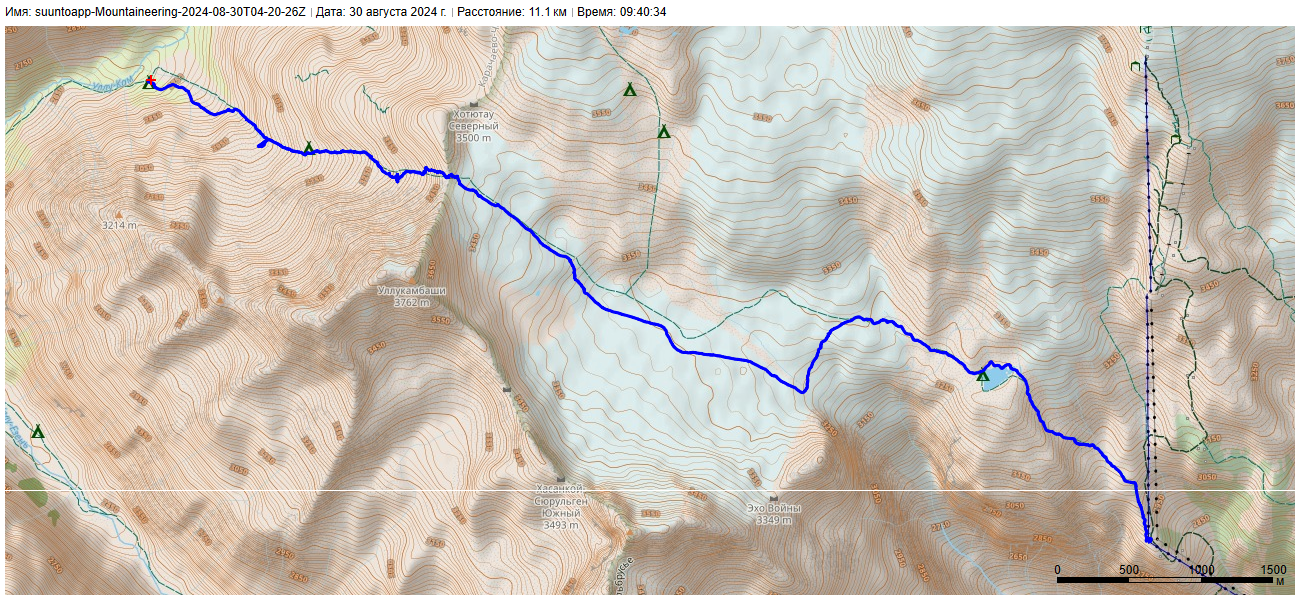
\includegraphics[angle=0, width=0.7\linewidth]{../pics/mini_maps/30}
	\label{fig:mini_30}
\end{figure}





Мы проснулись утром рано в 05:30. Позавтракали двойной порцией сухого омлета и отправились в путь в 07:20.

\begin{figure}[h!]
	\centering
	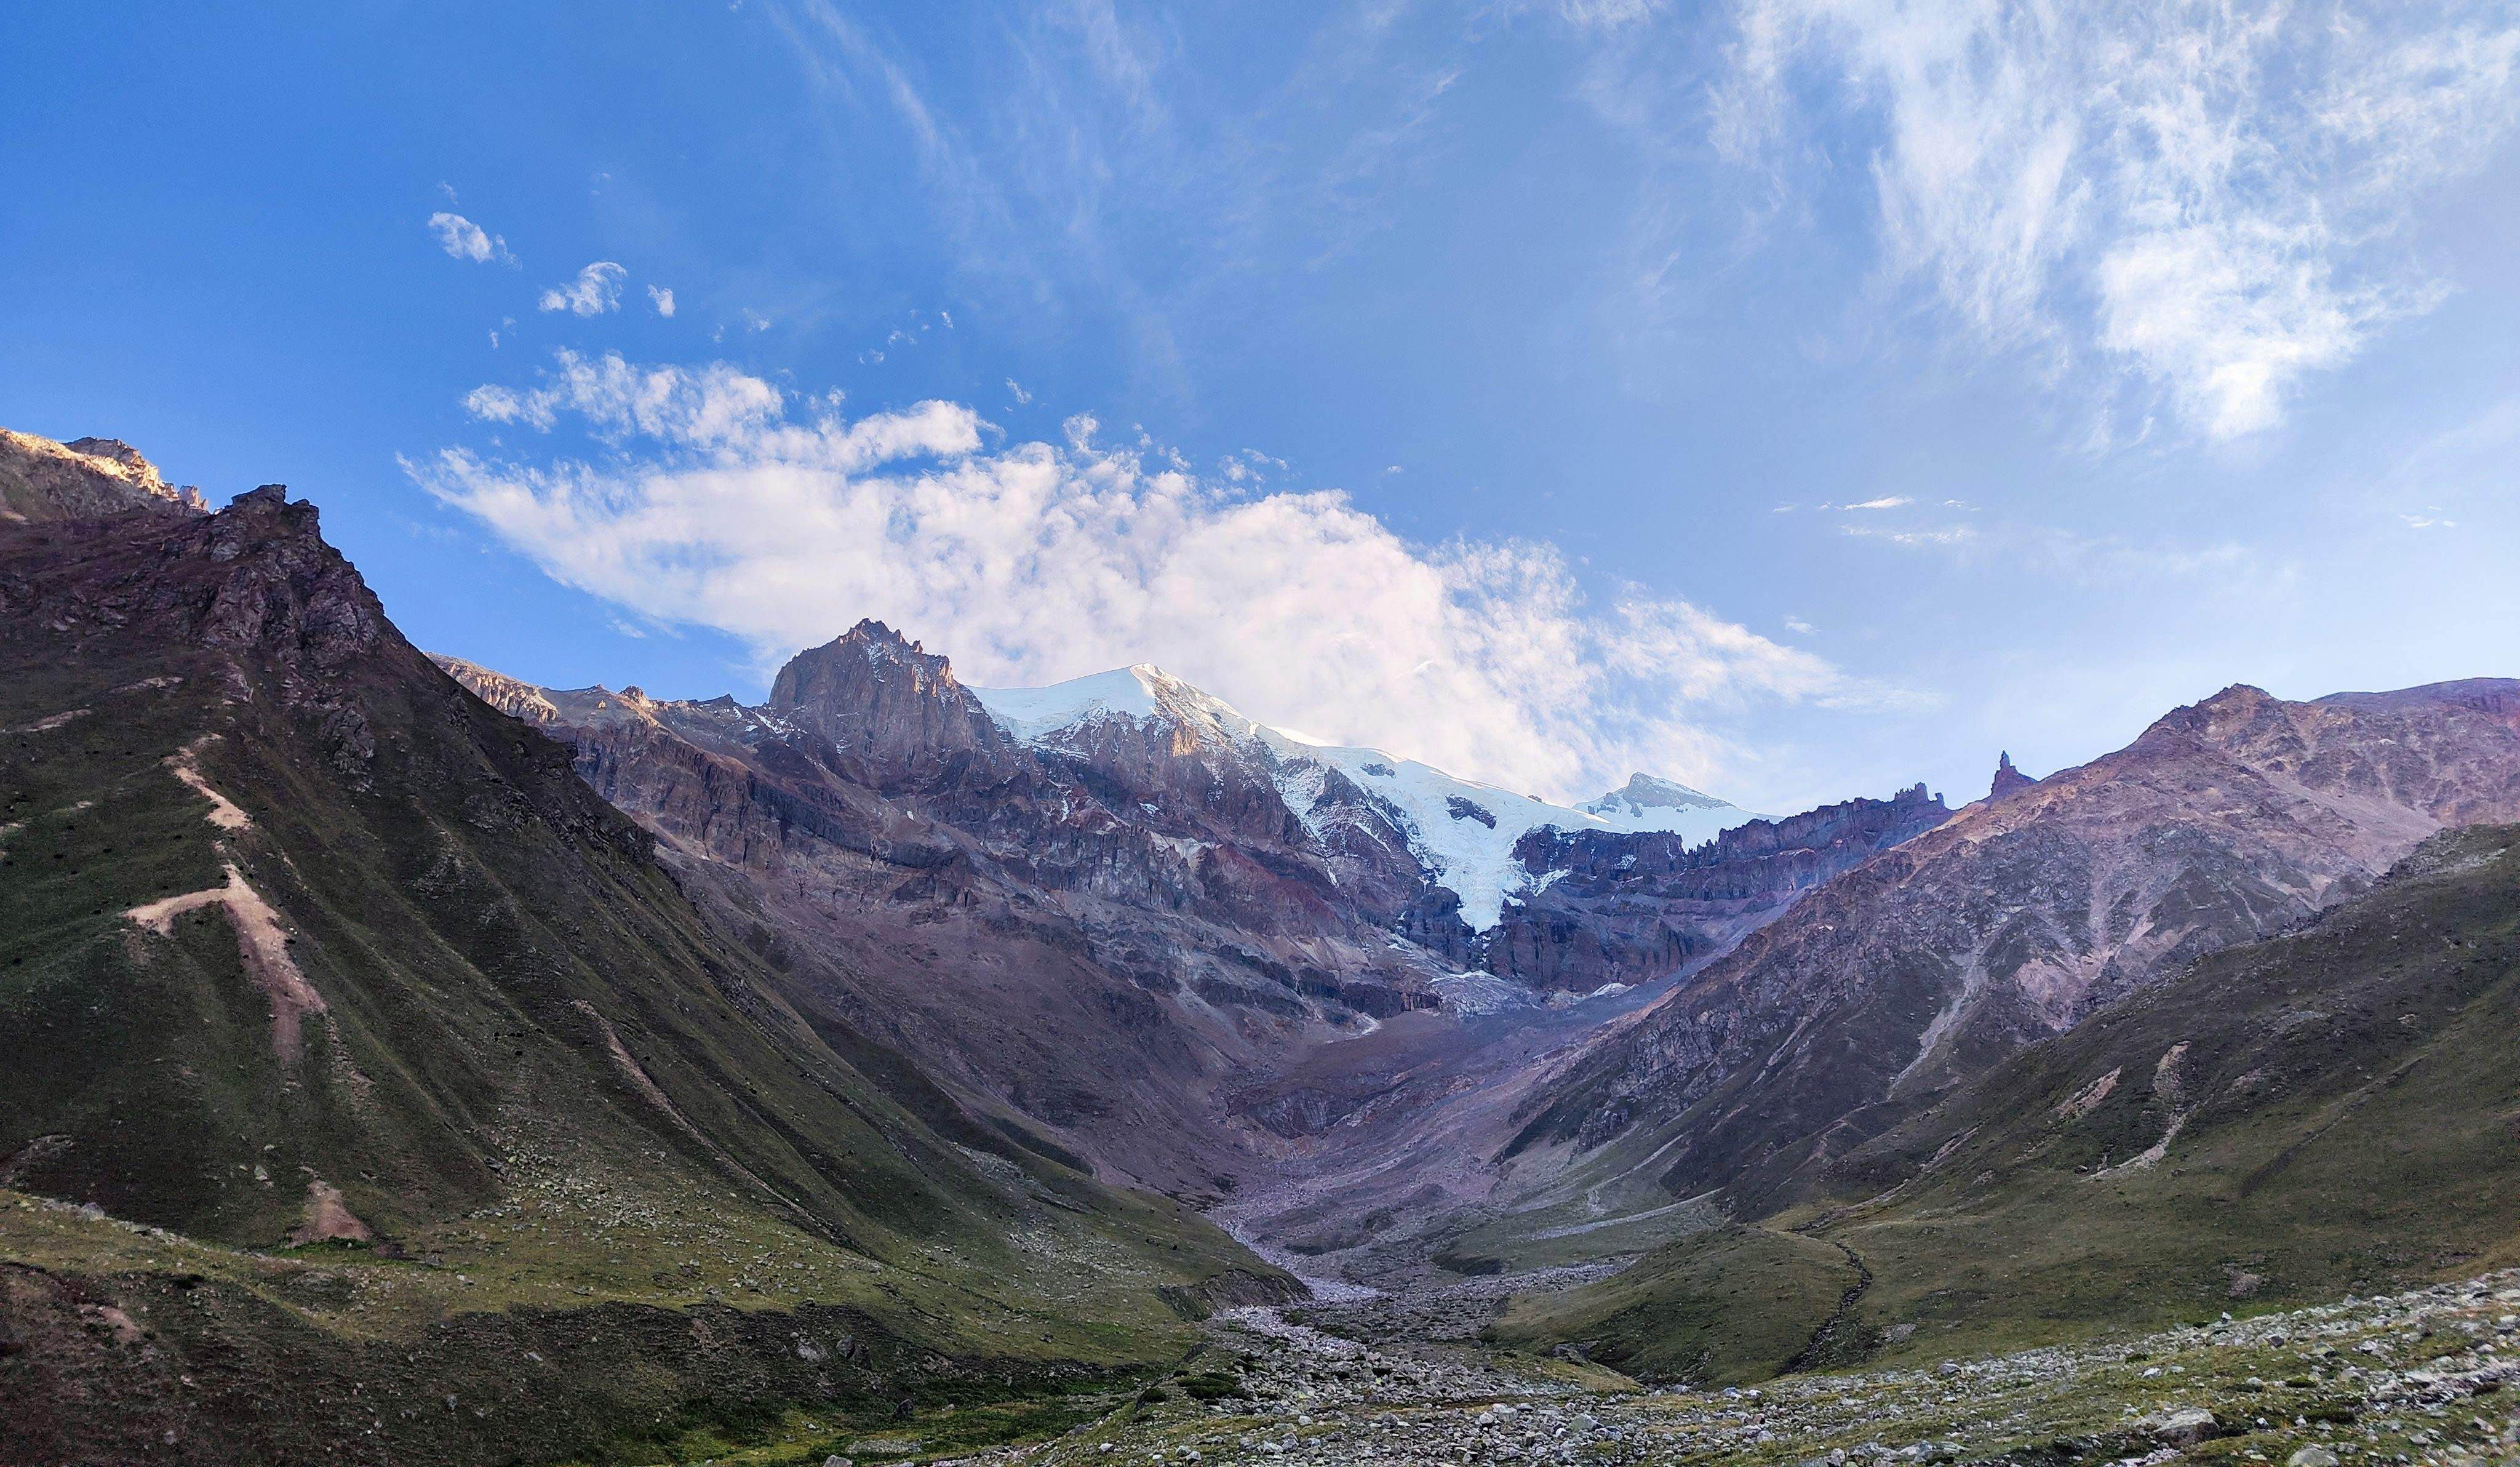
\includegraphics[width=0.7\linewidth]{../pics/IMG_20240830_063548}
	\caption{Утренний вид на юго-западные склоны Эльбруса}
	\label{fig:IMG_20240830_063548}
\end{figure}

До перевала ползли без особых проблем~--- сыпуха и курумник к концу похода стали нам родными и знакомыми. Путь технически и физически не сложный, но морально несколько утомляет, так как необходимо набрать 800 м высоты. Огромной поддержкой оказались синие метки трека для трейлраннеров Alpindustria Elbrus Race. Они значительно сократили нам время на поиск пути. Снег на перевальном взлёте отсутствует.

\begin{figure}[h!]
	\centering
	\begin{minipage}[h]{0.52\linewidth}
		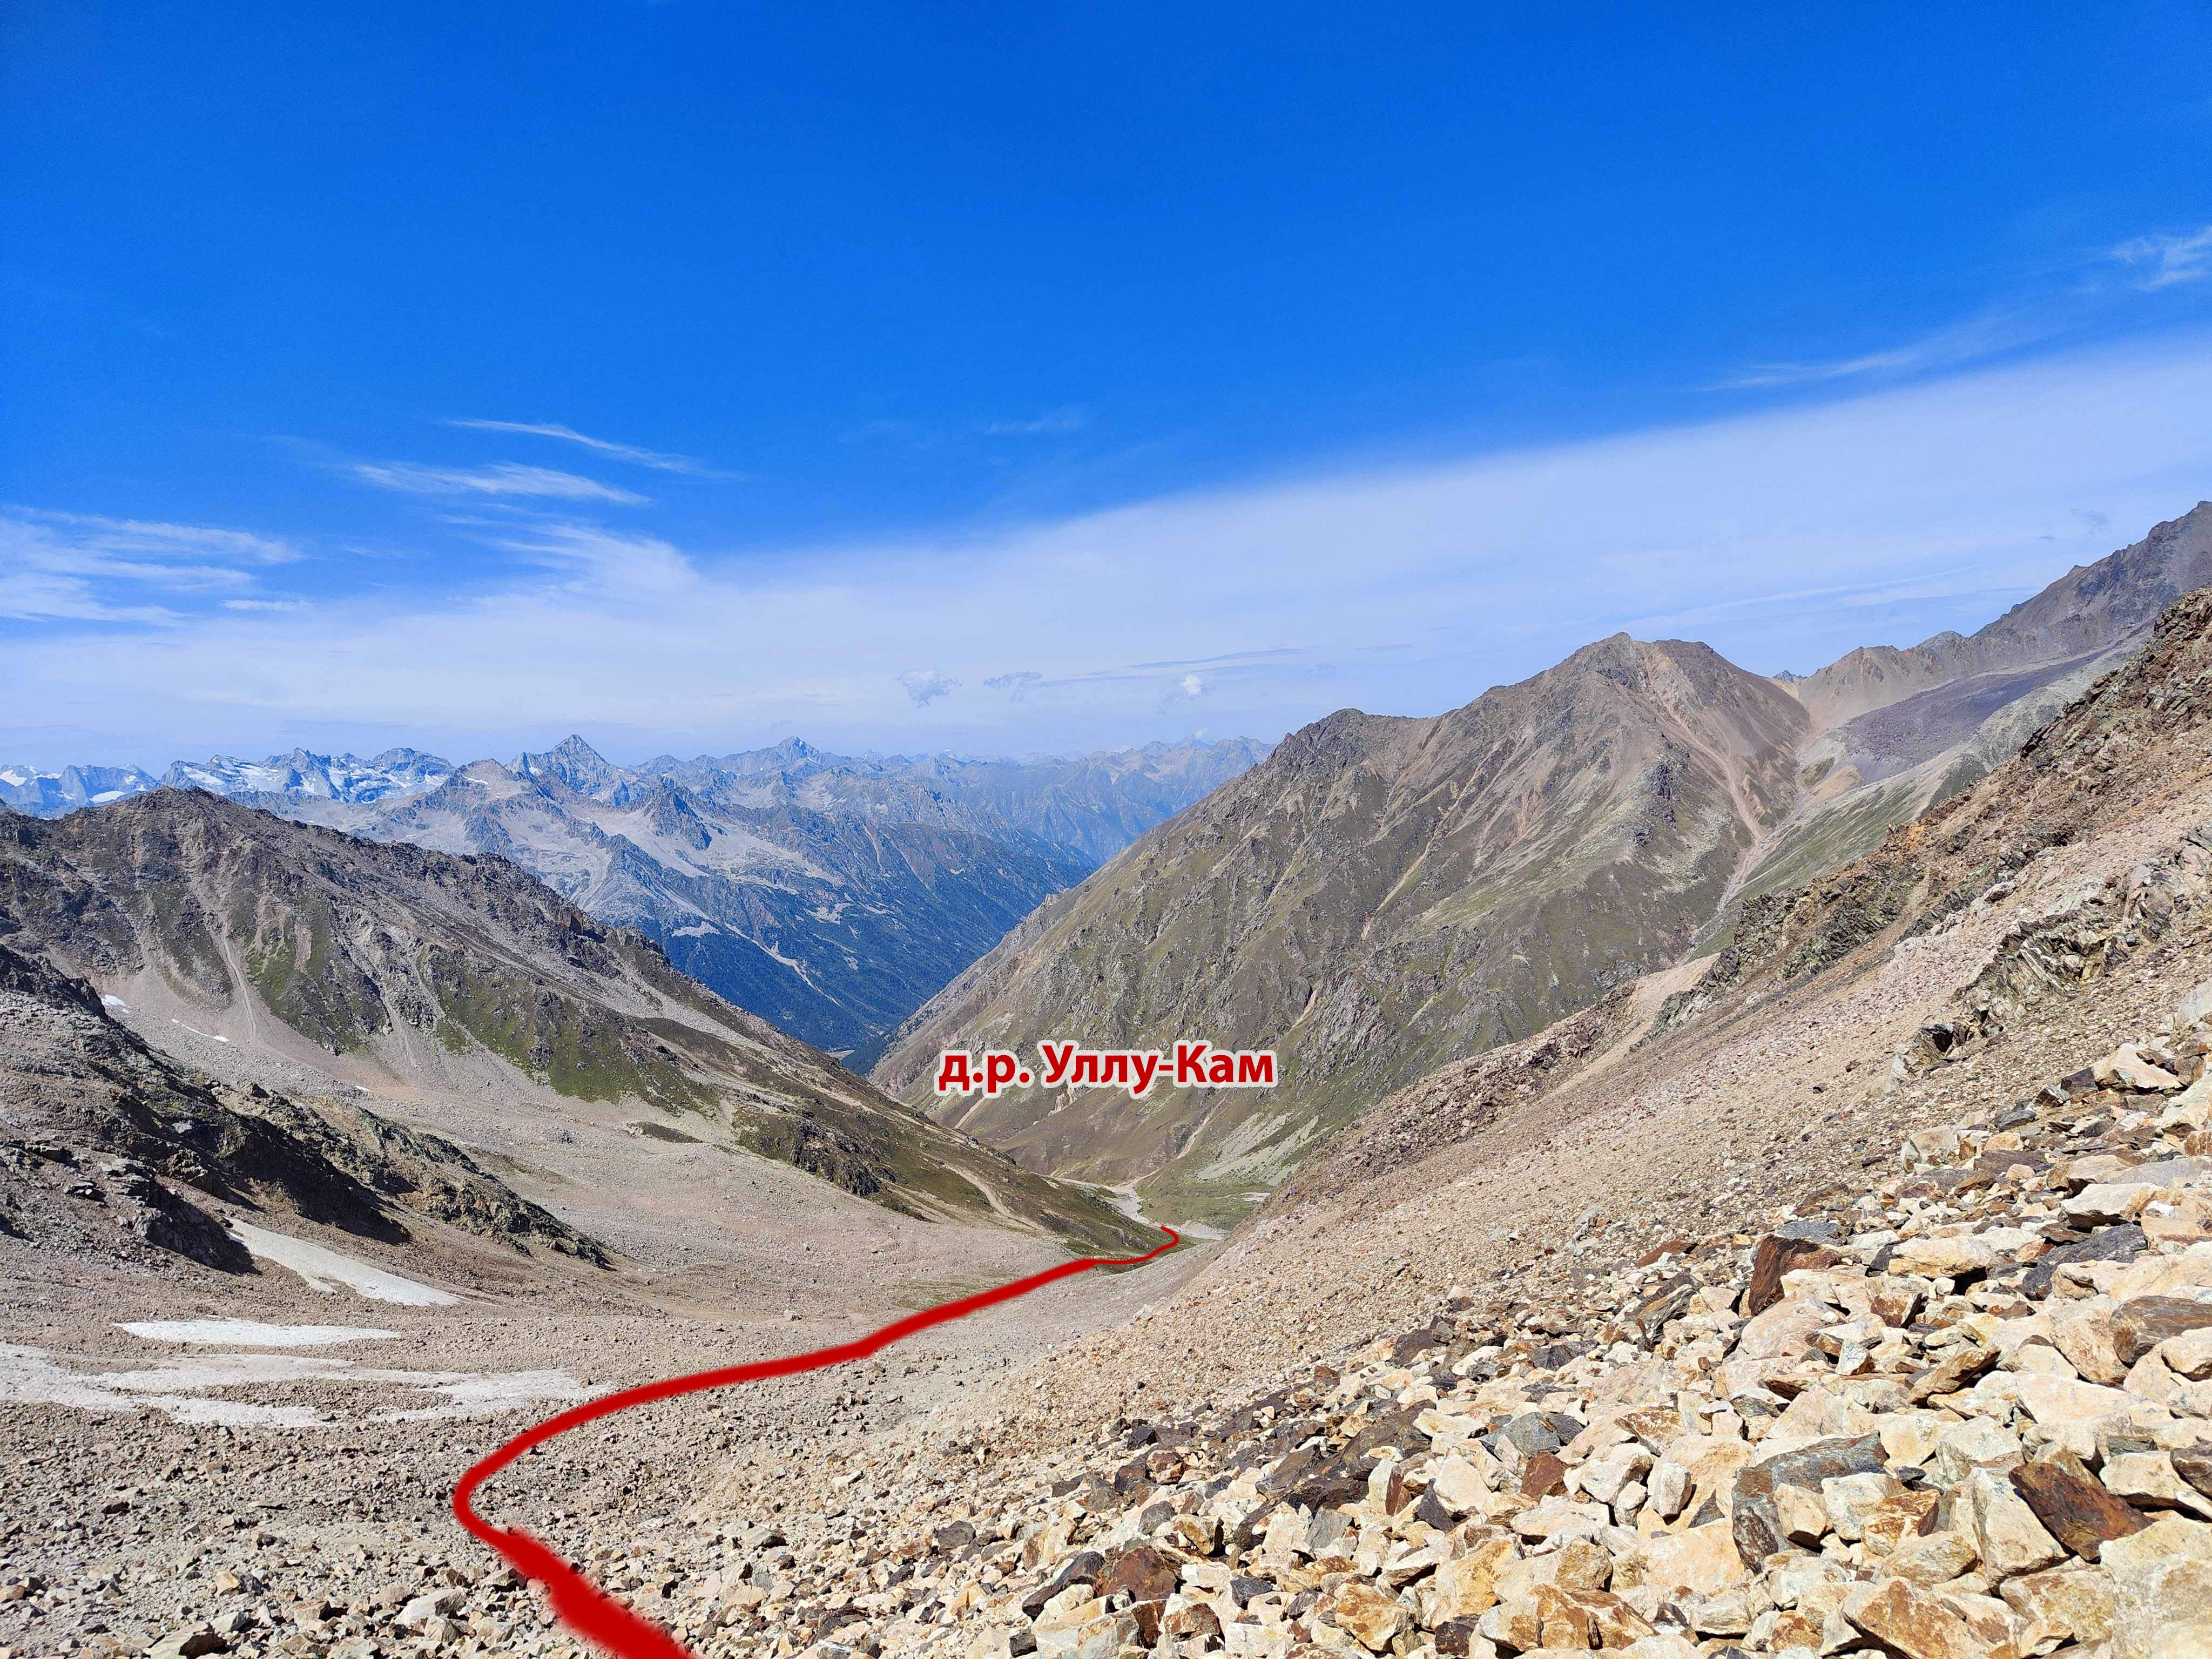
\includegraphics[width=0.99\linewidth]{../pics/IMG_20240830_105443}
	\end{minipage}
	\qquad
	\begin{minipage}[h]{0.29\linewidth}
		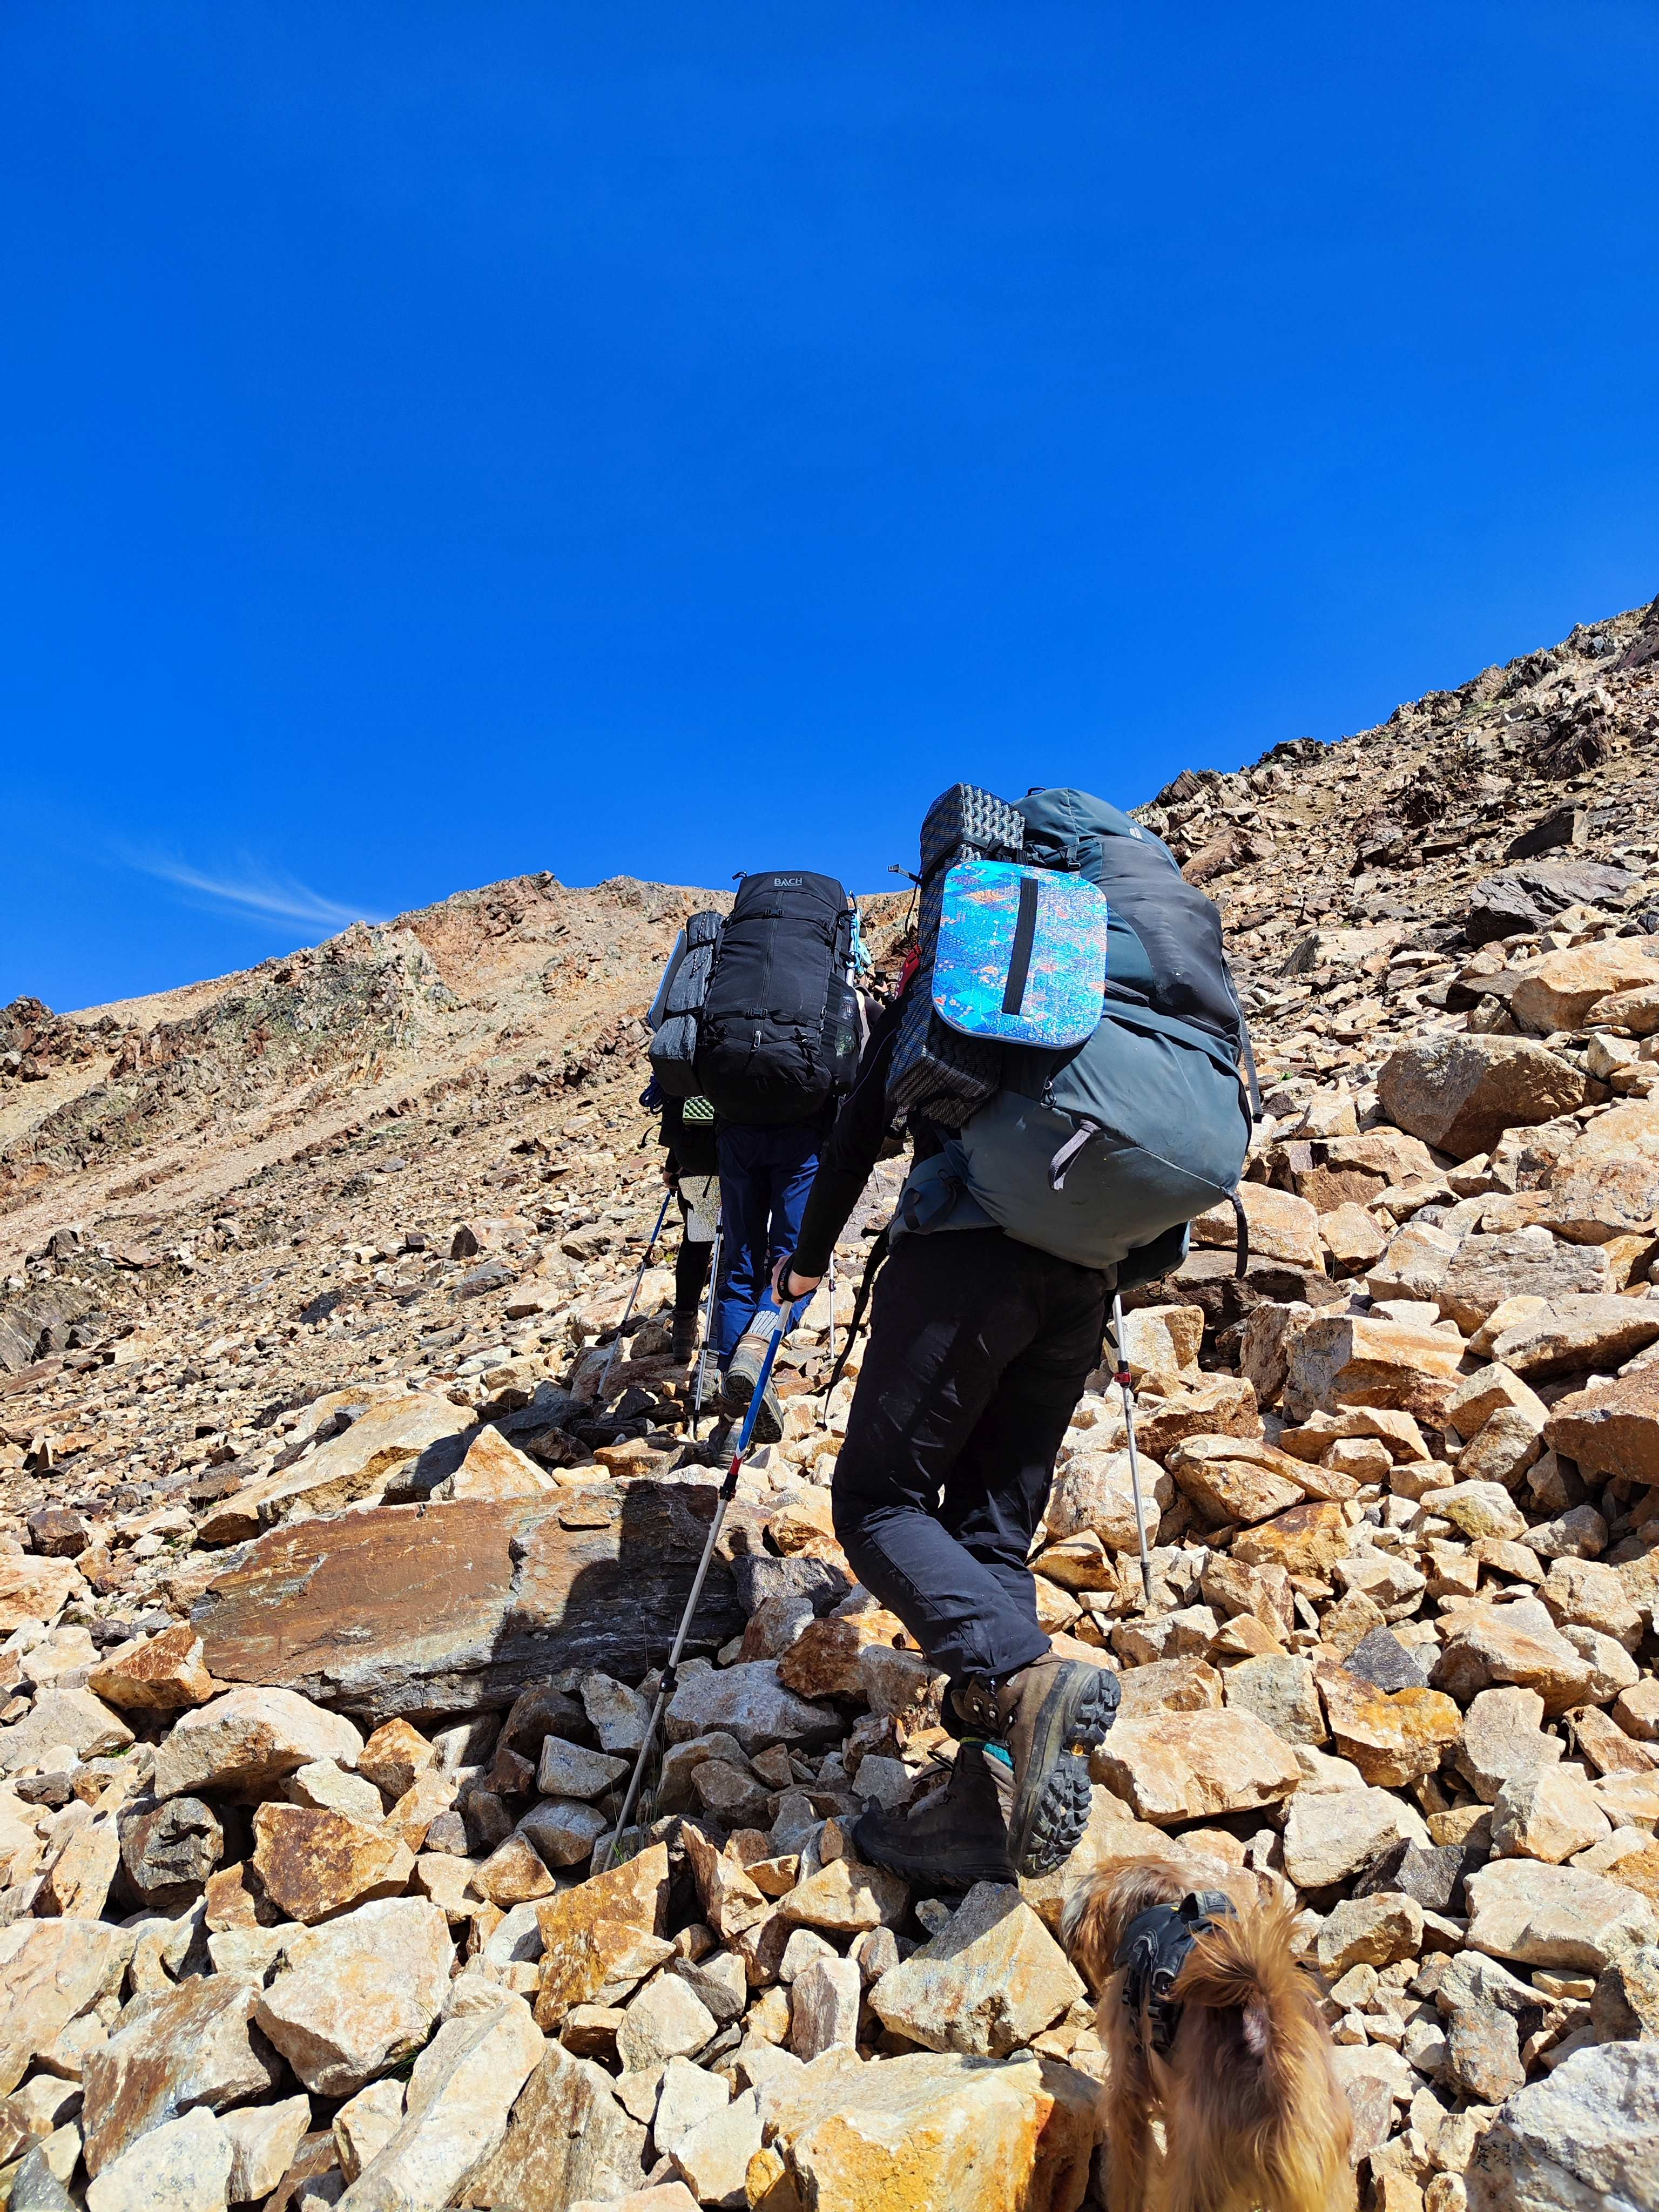
\includegraphics[width=0.99\linewidth]{../pics/IMG_20240830_105447}
	\end{minipage}
	\caption{Слева: вид на путь подъёма. Справа: поднимаемся на перевал}
	\label{fig:IMG_20240830_105443}
\end{figure}

В 11:30 поднимаемся на перевал. Погода шикарная, открываются потрясающие виды на горы Карачаево-Черкессии, Кабардино-Балкарии и, конечнно, Эльбрус. Ледник Большой Азау открыт. Много памятных табличек, восвящённых военным действиям в годы ВОВ. Фотографируемся, отзваниваемся и отписываемся родным, радуемся малому количеству мусора на перевале (судя по отчётам, с этим были проблемы). Снимаем две перевальные записки~--- проекта <<Виртуальные горы>> от 28.08.2024 и турклуба <<ЛИИЖТ>> г. Санкт-Петербург от 21.08.2024.

\begin{figure}[h!]
	\centering
	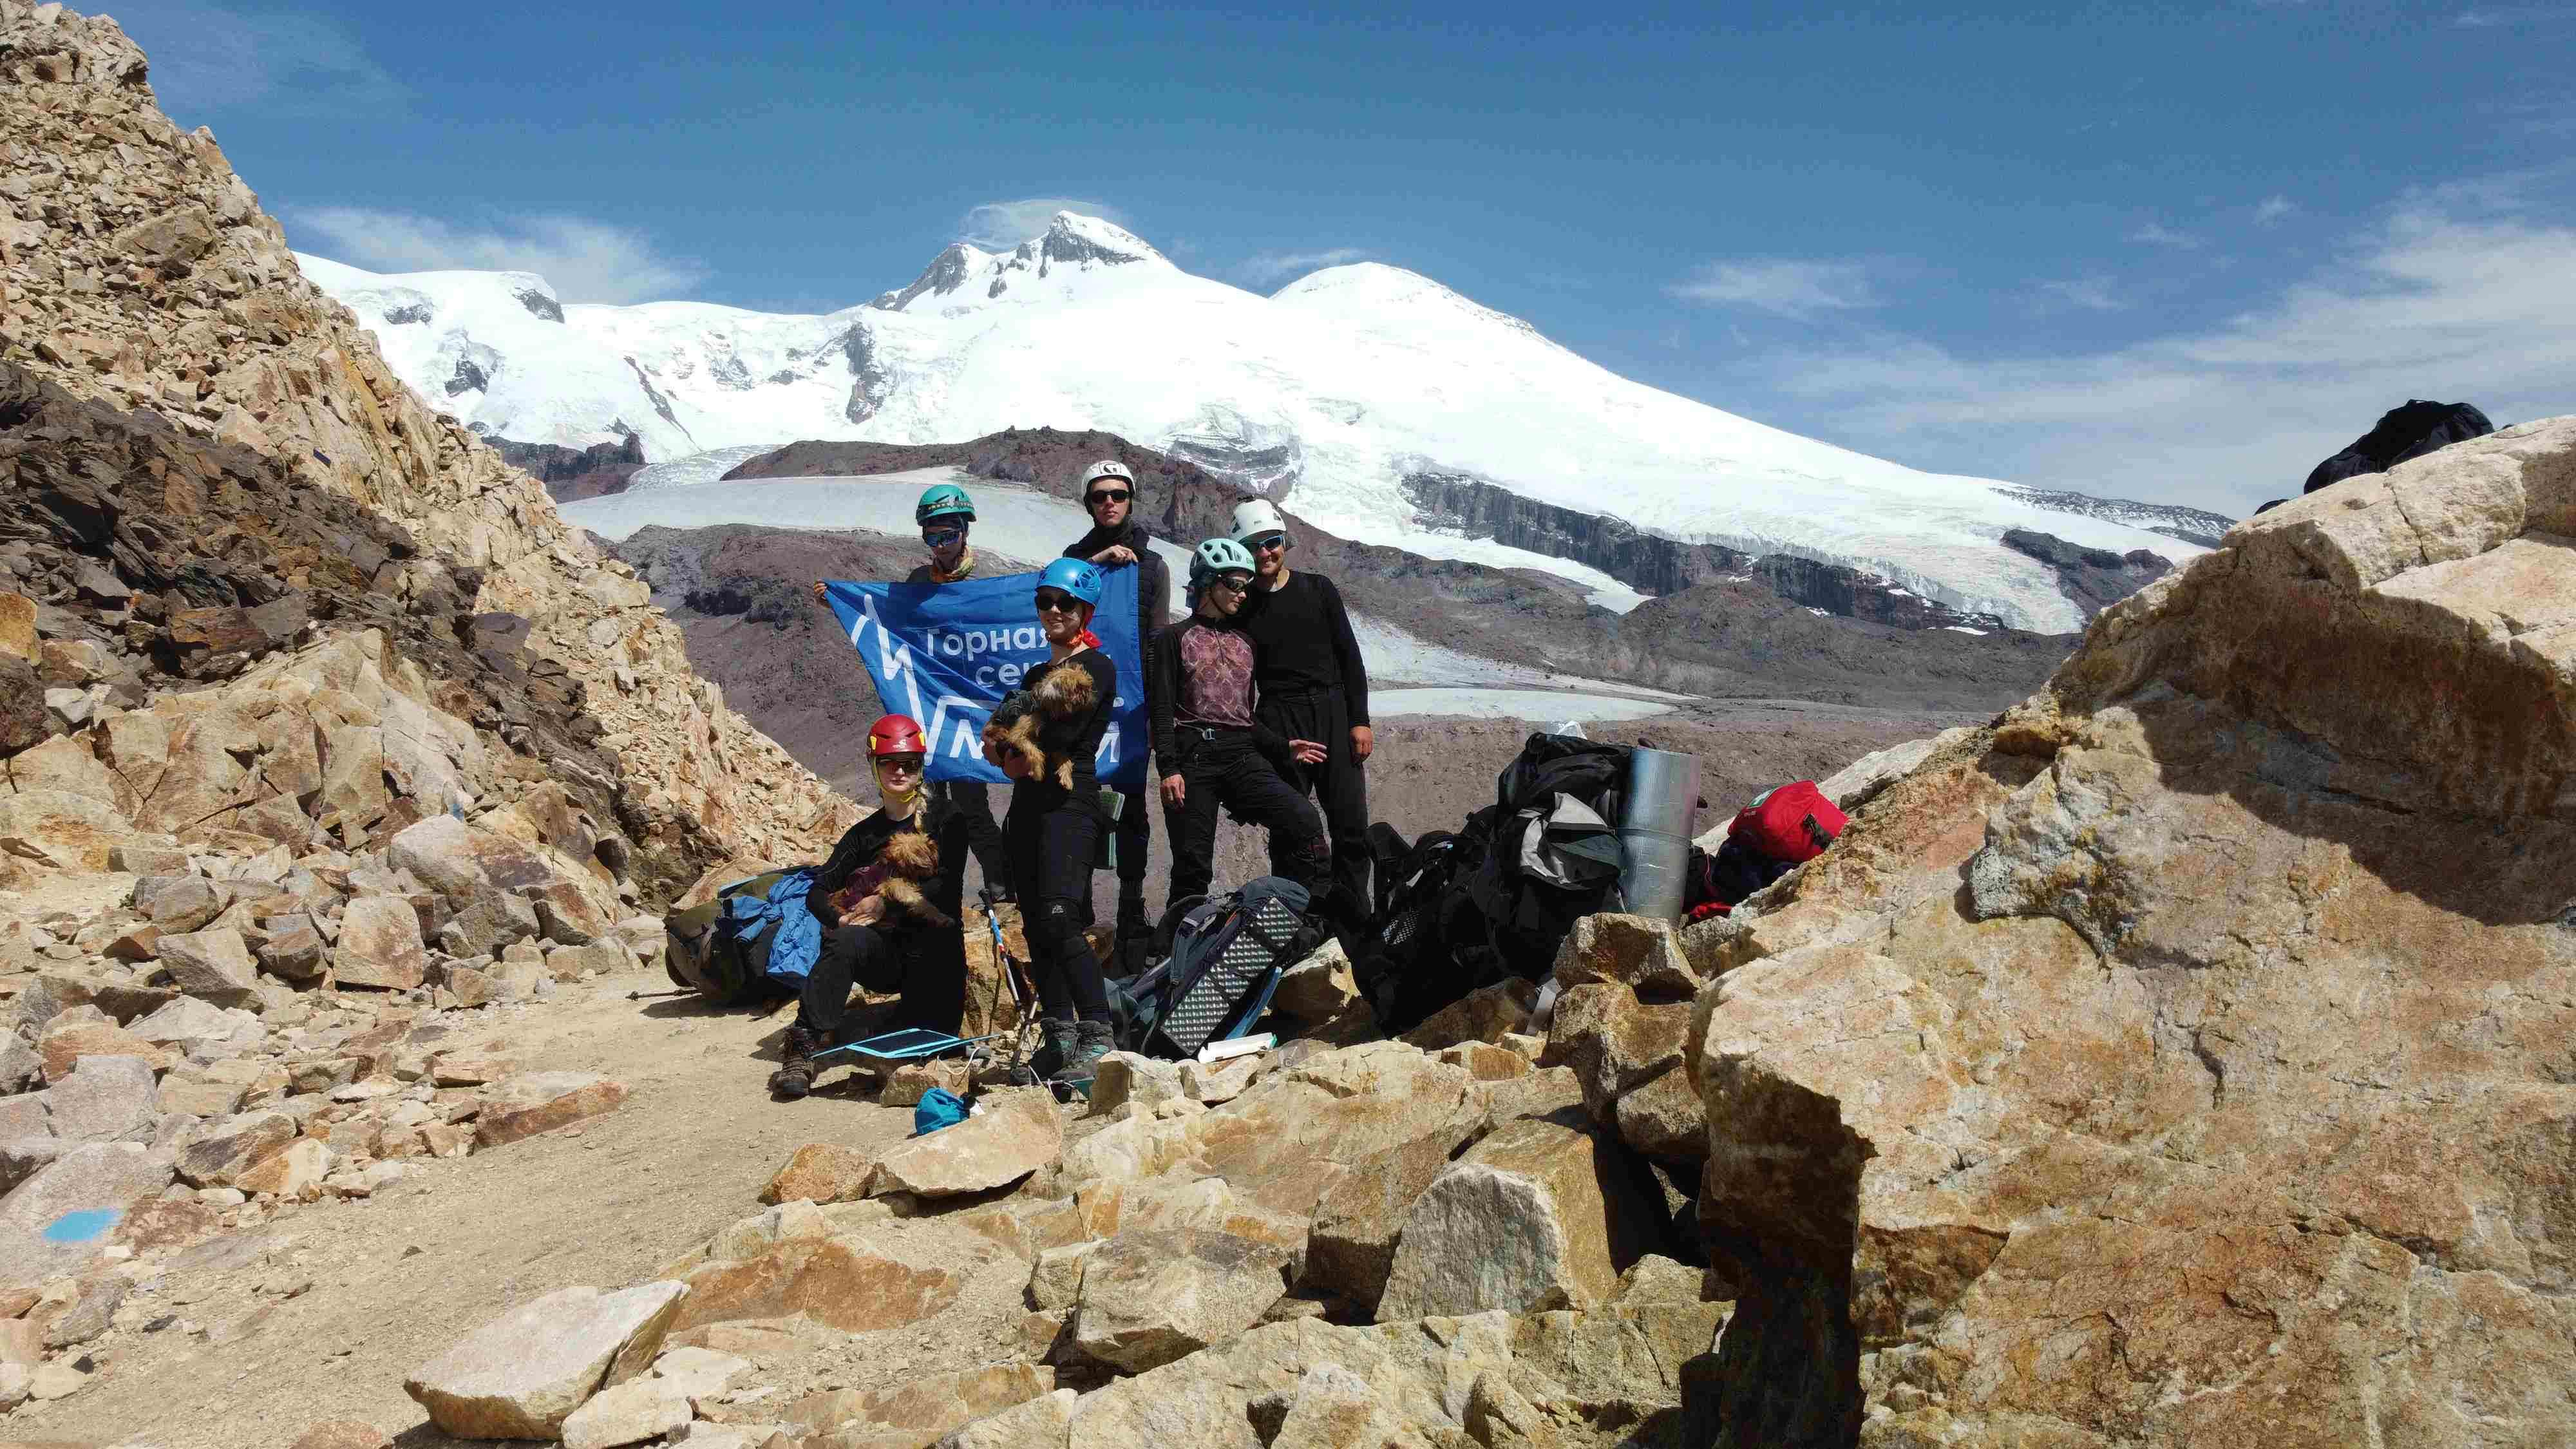
\includegraphics[width=0.7\linewidth]{../pics/DJI_0899}
	\caption{группа на пер. Хотютау}
	\label{fig:hotyutau_1}
\end{figure}

В 12:30 начинаем спуск. На ледник спуск идёт по мелкой сыпухе, в связи с чем пытаемся показать группе спуск <<лифтом>>. В 12:49 оказываемся на леднике. Обнаруживаем на седловине перевала двух туристов, надеваем кошки и начинаем движение по леднику. Поскольку ледник был, трещины хорошо просматривались и легко обходились.

\begin{figure}[h!]
	\centering
	\begin{minipage}[h]{0.4\linewidth}
		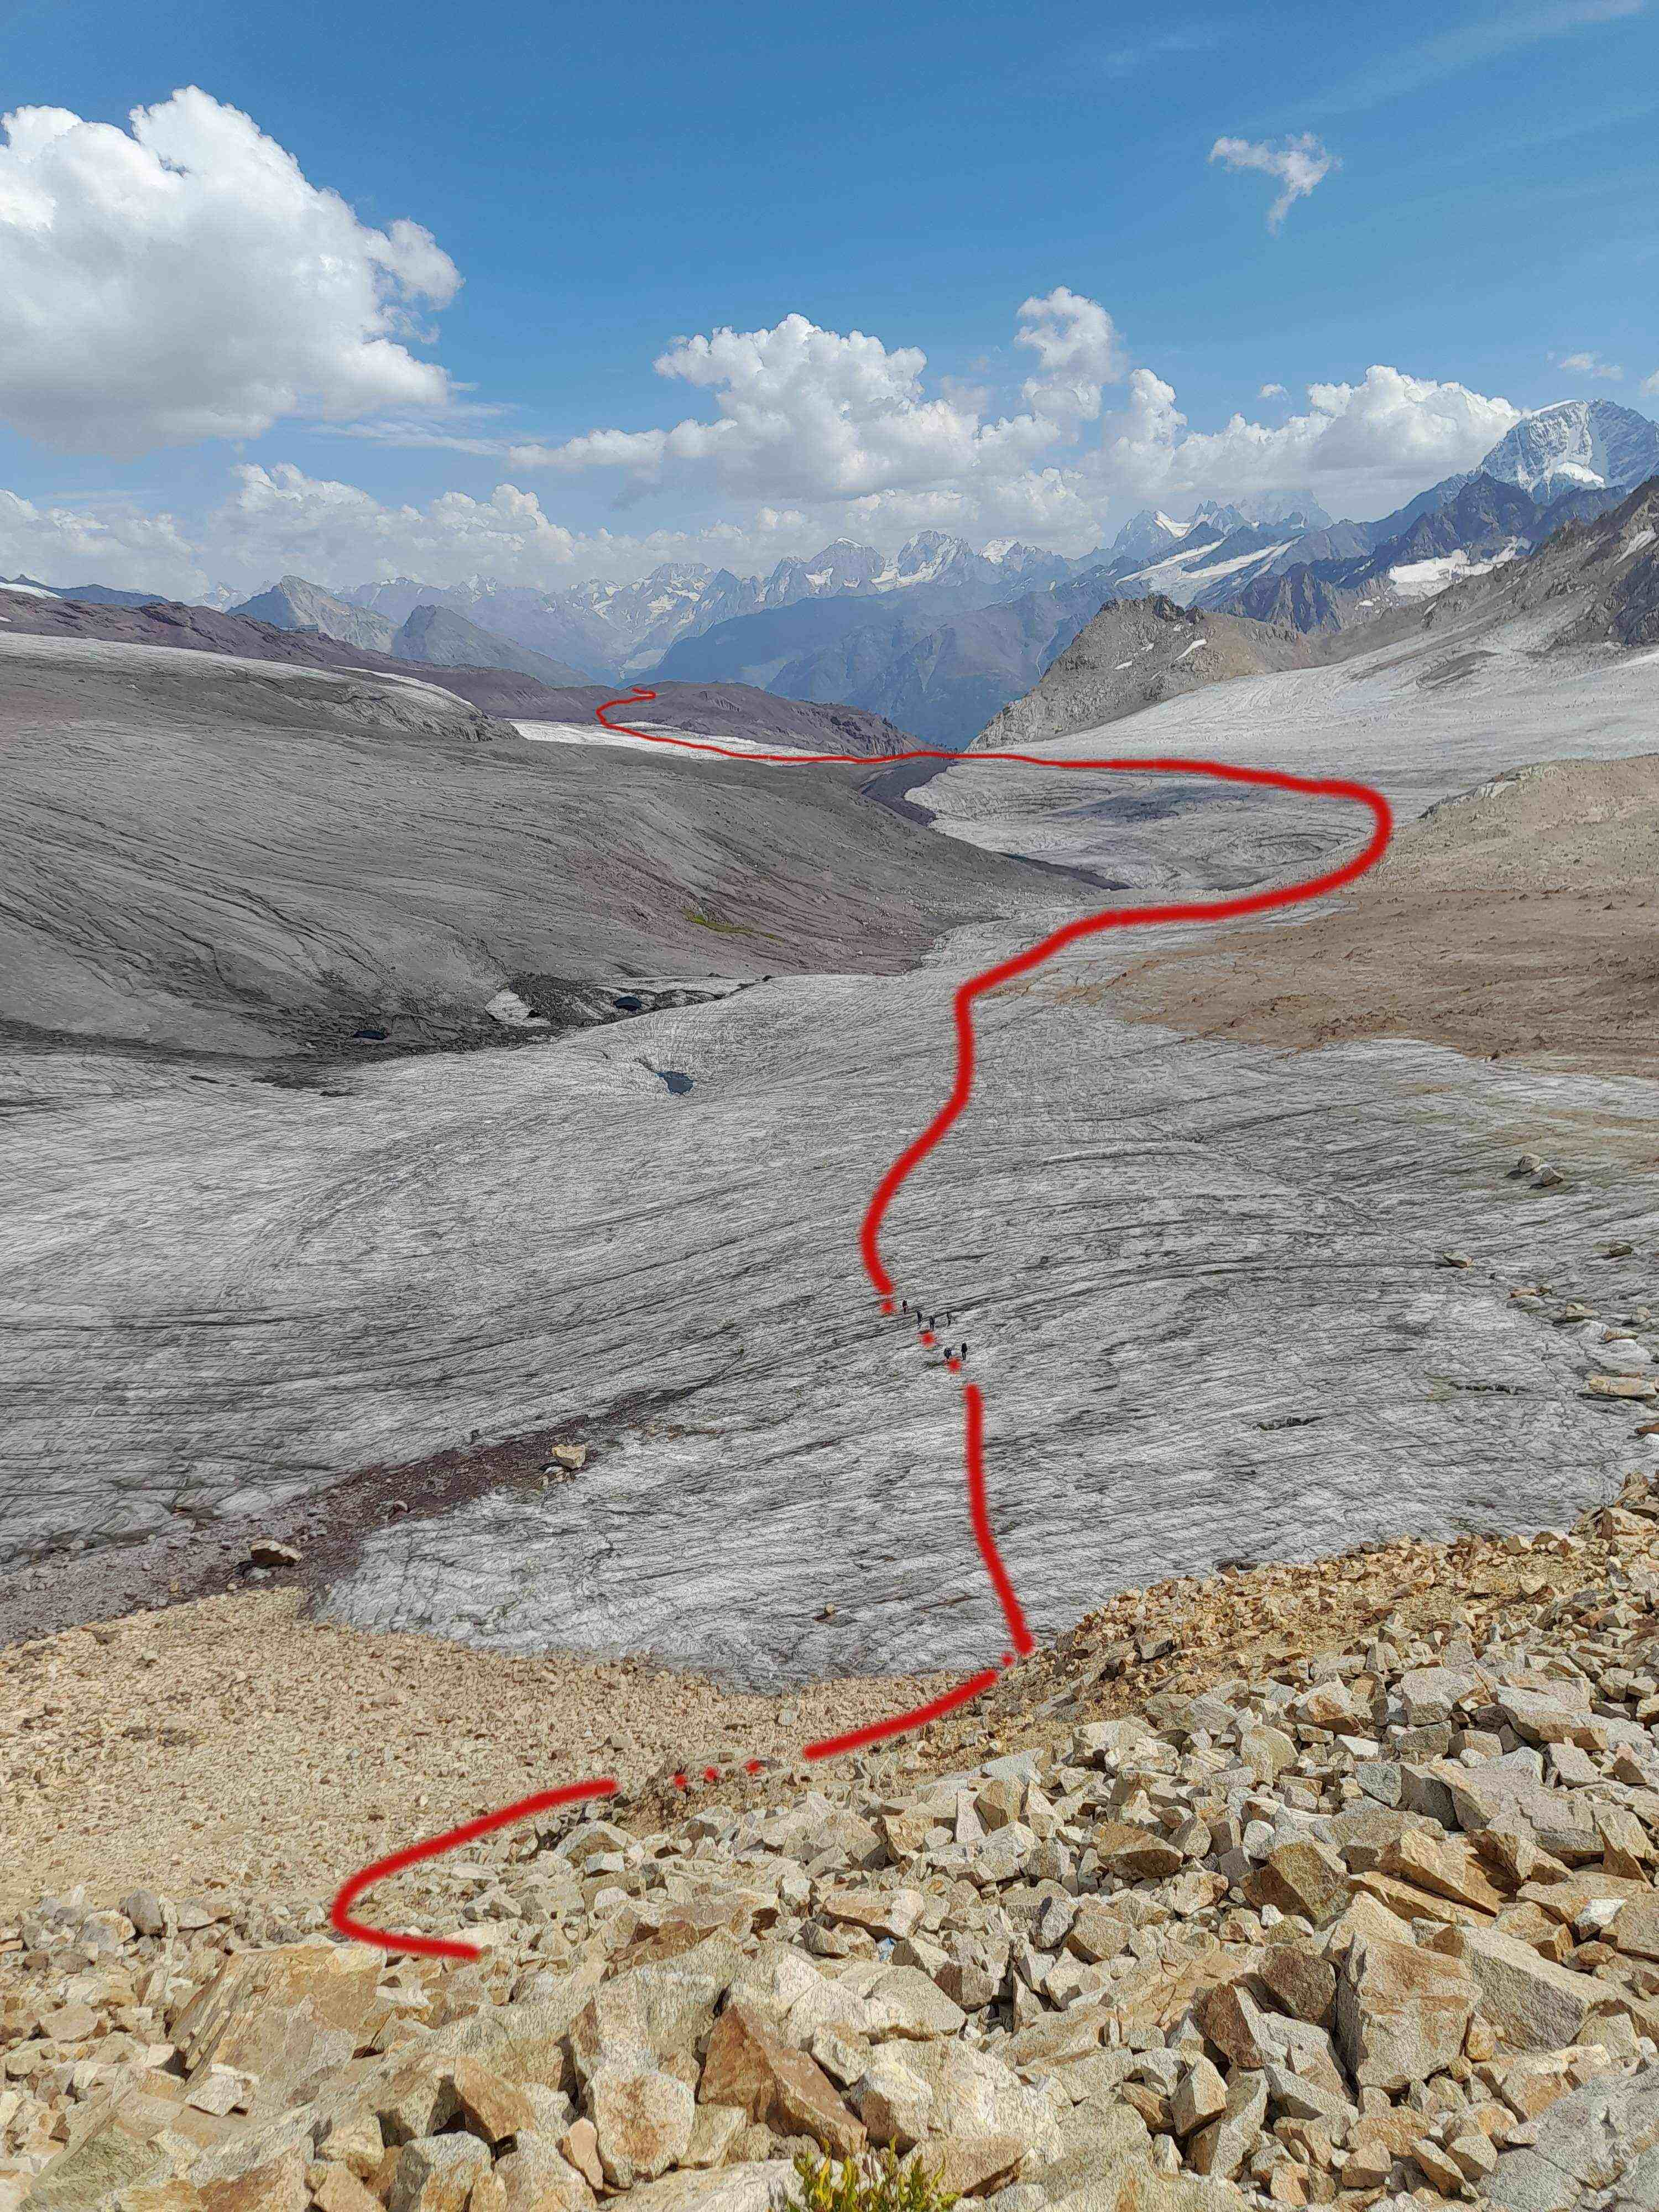
\includegraphics[width=0.99\linewidth]{../pics/20240830_141852.jpg}
	\end{minipage}
	\qquad
	\begin{minipage}[h]{0.4\linewidth}
		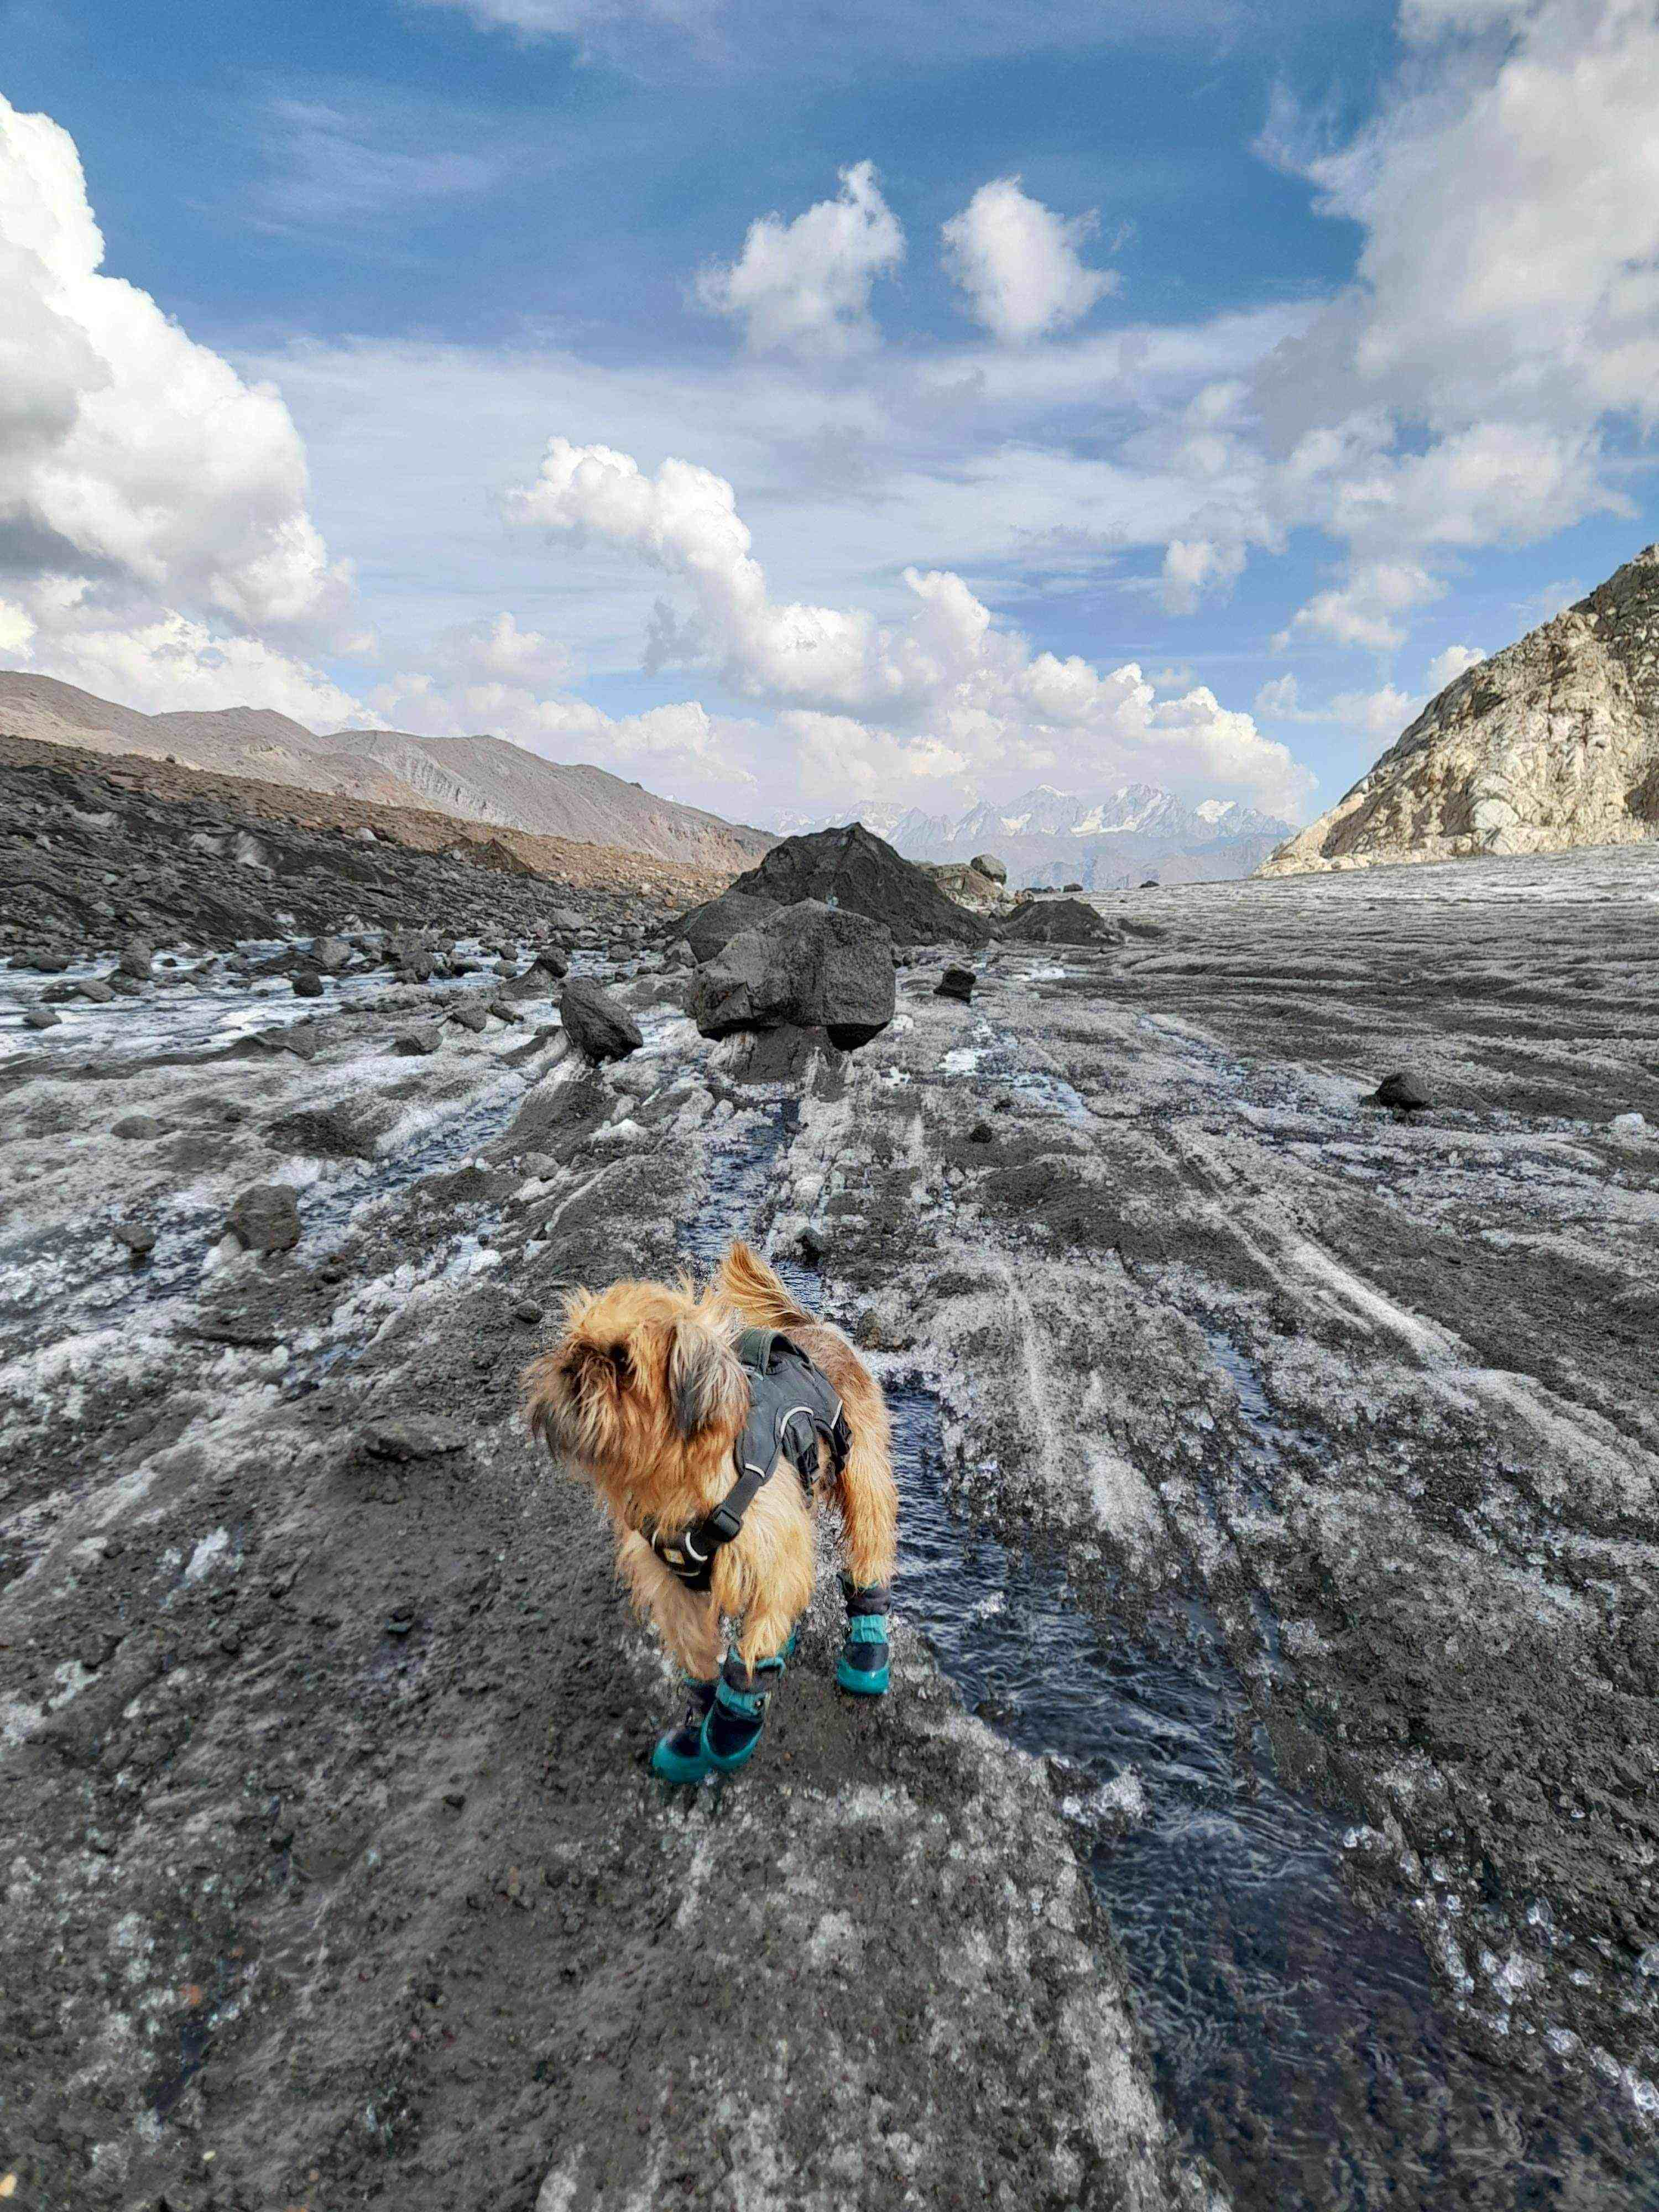
\includegraphics[width=0.99\linewidth]{../pics/20240830_155136.jpg}
	\end{minipage}
	\caption{Слева: группа на леднике. Фото туристов т/к МАИ. Справа: единственный раз, когда собакам действительно пригодились ботинки~--- это переход по леднику}
	\label{fig:20240830_141852}
\end{figure}

На ближайшем привале нас догоняют туристы горной секции МАИ. Как выяснилось, оставленная нами записка пролежала в камнях не более получаса. Увеличенным составом мы двигаемся по ледник и таки допускаем досадную ошибку, пройдя мимо <<красной>> и <<чёрной>> морен и забыв вовремя свернуть налево. Поворачиваем в нужную сторону в 15:00. Из-за этого пришлось набирать лишние 50~м высоты. На ледовые поля ложится плотный туман, поэтому мы были очень рады, когда, наконец, увидели на моренах знакомую синюю метку. По хорошо протоптанной дорожке далее идём без проблем. 

В 16:20 выходим к Эльбрусскому озеру. Решаем обойти его по северному берегу, хотя, стоит заметить, что трейлраннинговая тропа идёт по противоположному, южному берегу.

\begin{figure}[h!]
	\centering
	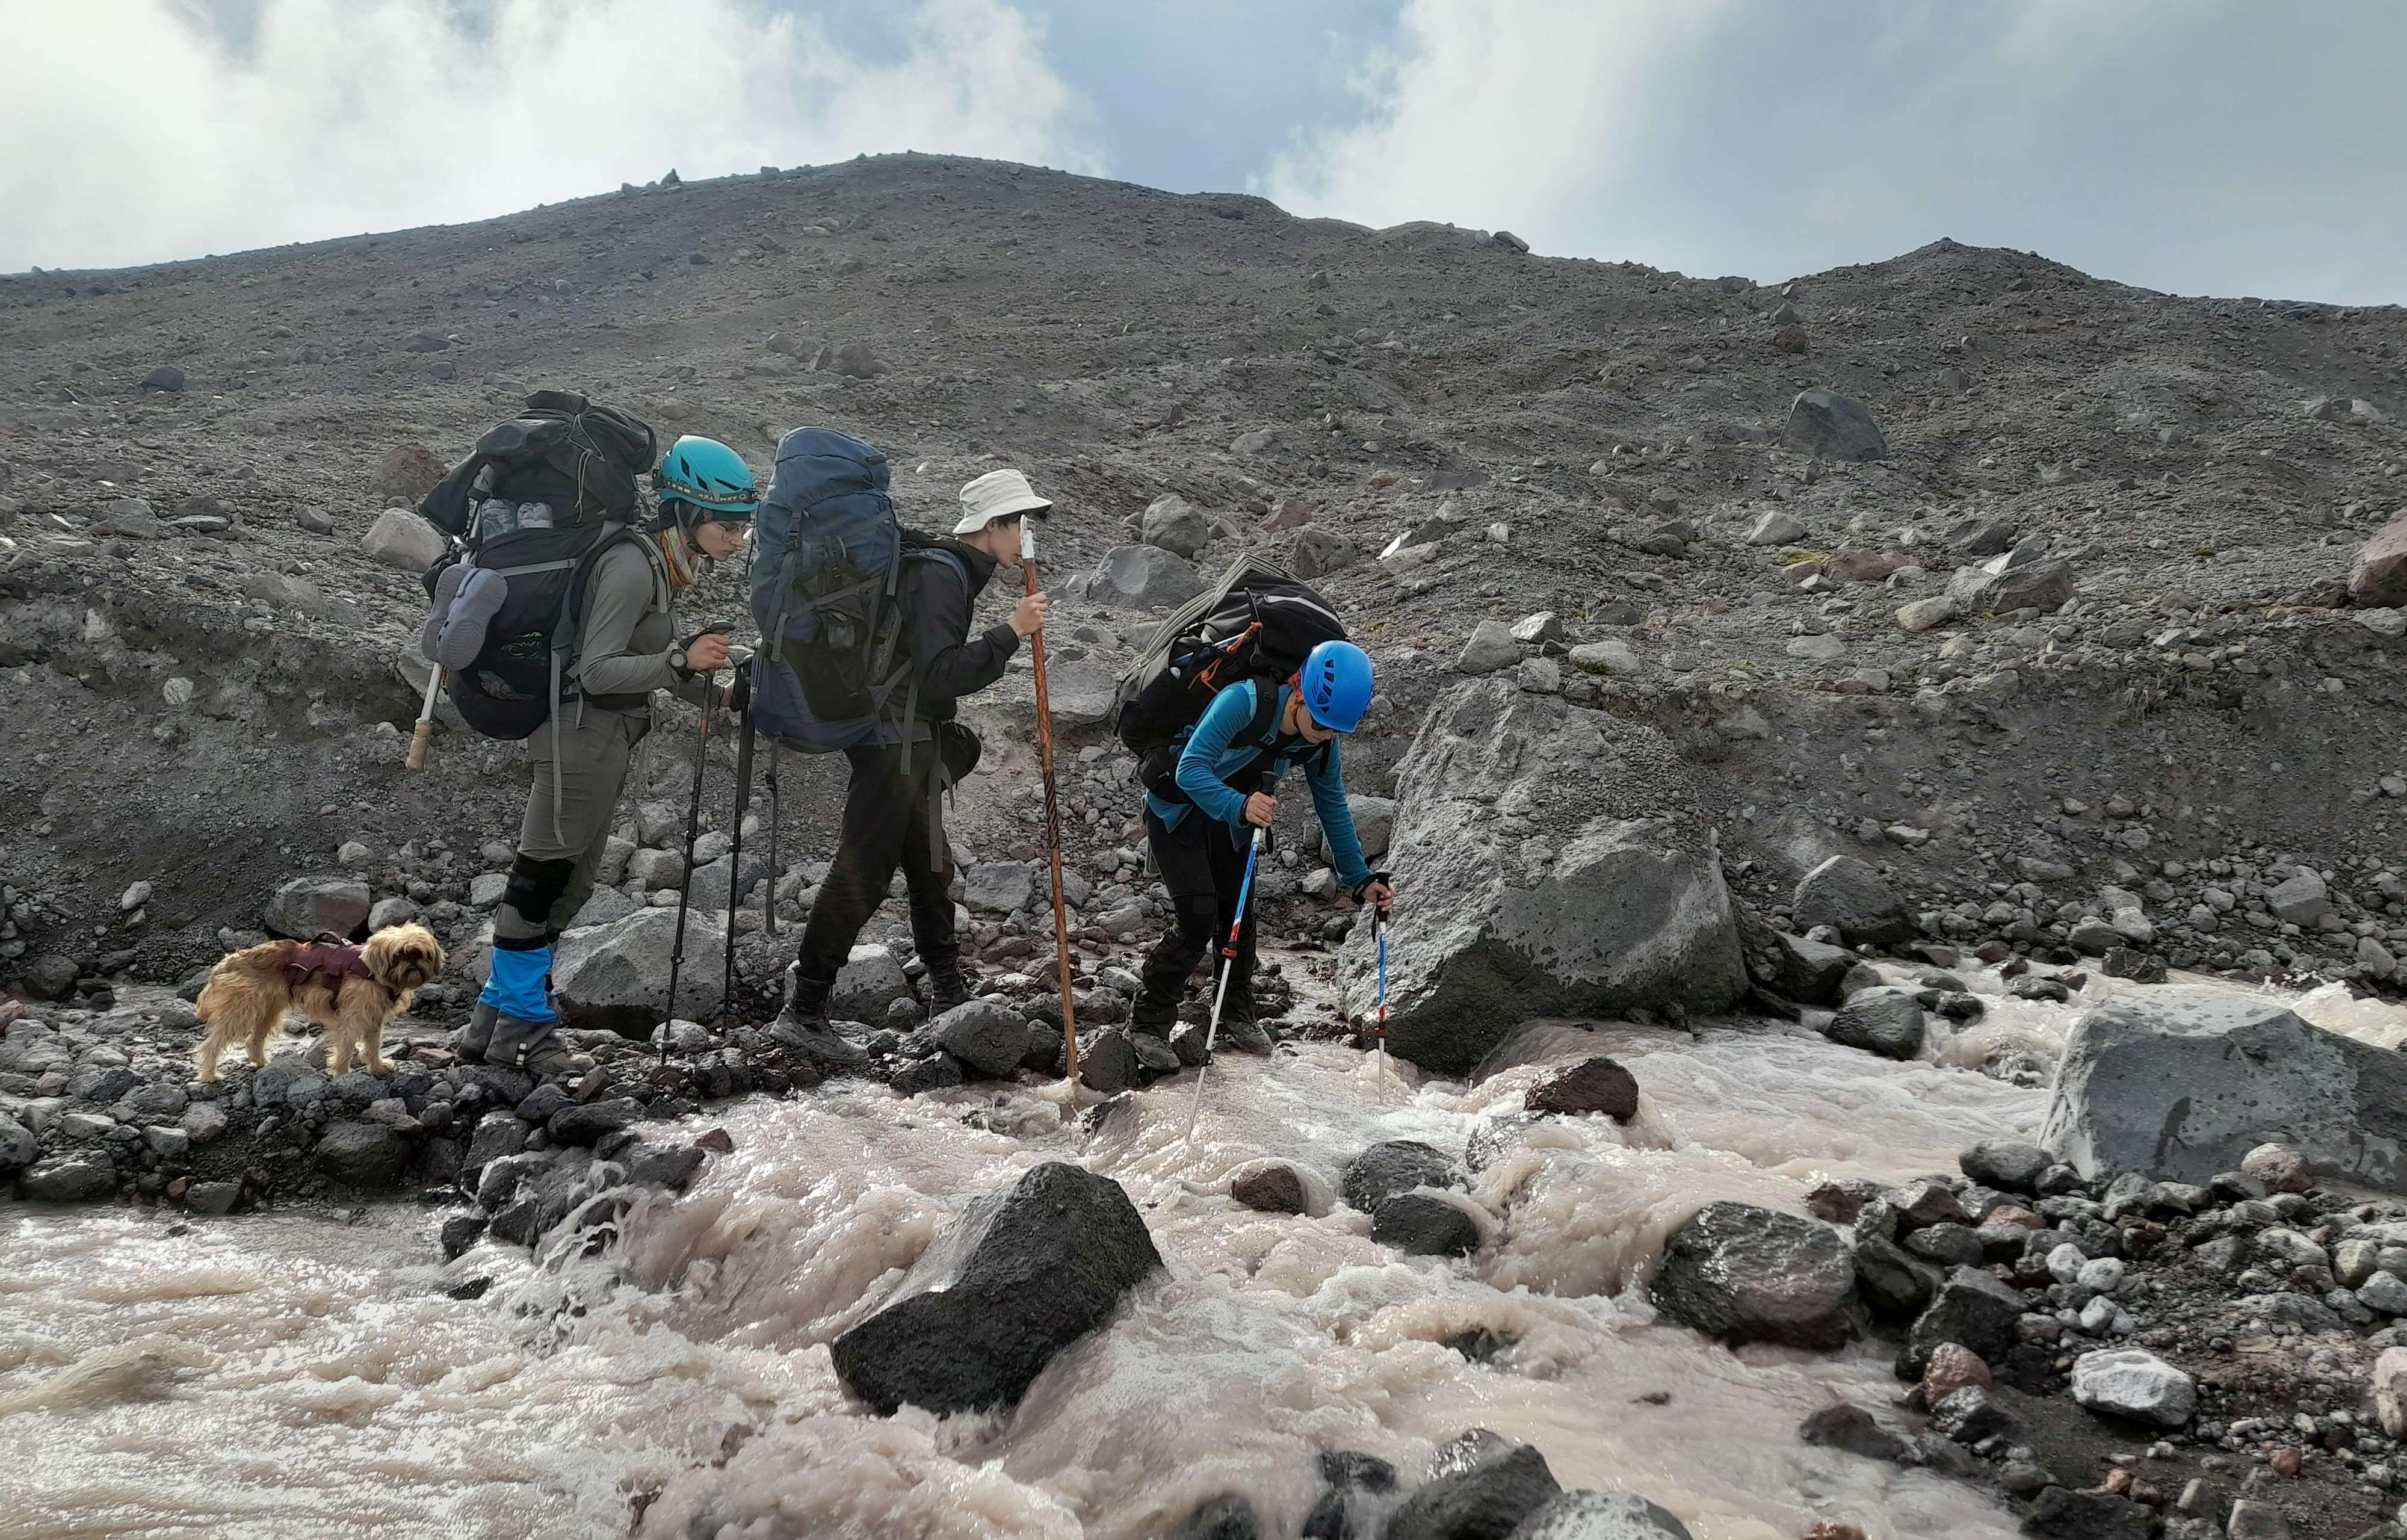
\includegraphics[width=0.7\linewidth]{../pics/20240830_162252.jpg}
	\caption{Бродим ручей, впадающий в Эльбрусское озеро}
	\label{fig:20240830_162252.jpg}
\end{figure}

В этот момент выясняется, что до закрытия канатной дороги остается меньше получаса. Остаток пути от озера до станции <<Кругозор>> представлят собой довольно крутой спуск. Сейчас он безопасен и хорошо оборудован, ибо, помимо протоптанной тропы и синей маркировки, имеются оборудованные мосты через ручьи и виа-ферраты на локальных крутых участках. Мы идём на всех парах, играя в трейлраннеров с рюкзаками за плечами: за 25 минут пробегаем 2 км со сбросом 310 м и садимся в кабинку канатной дороги ровно в 17:00.

\begin{figure}[h!]
	\centering
	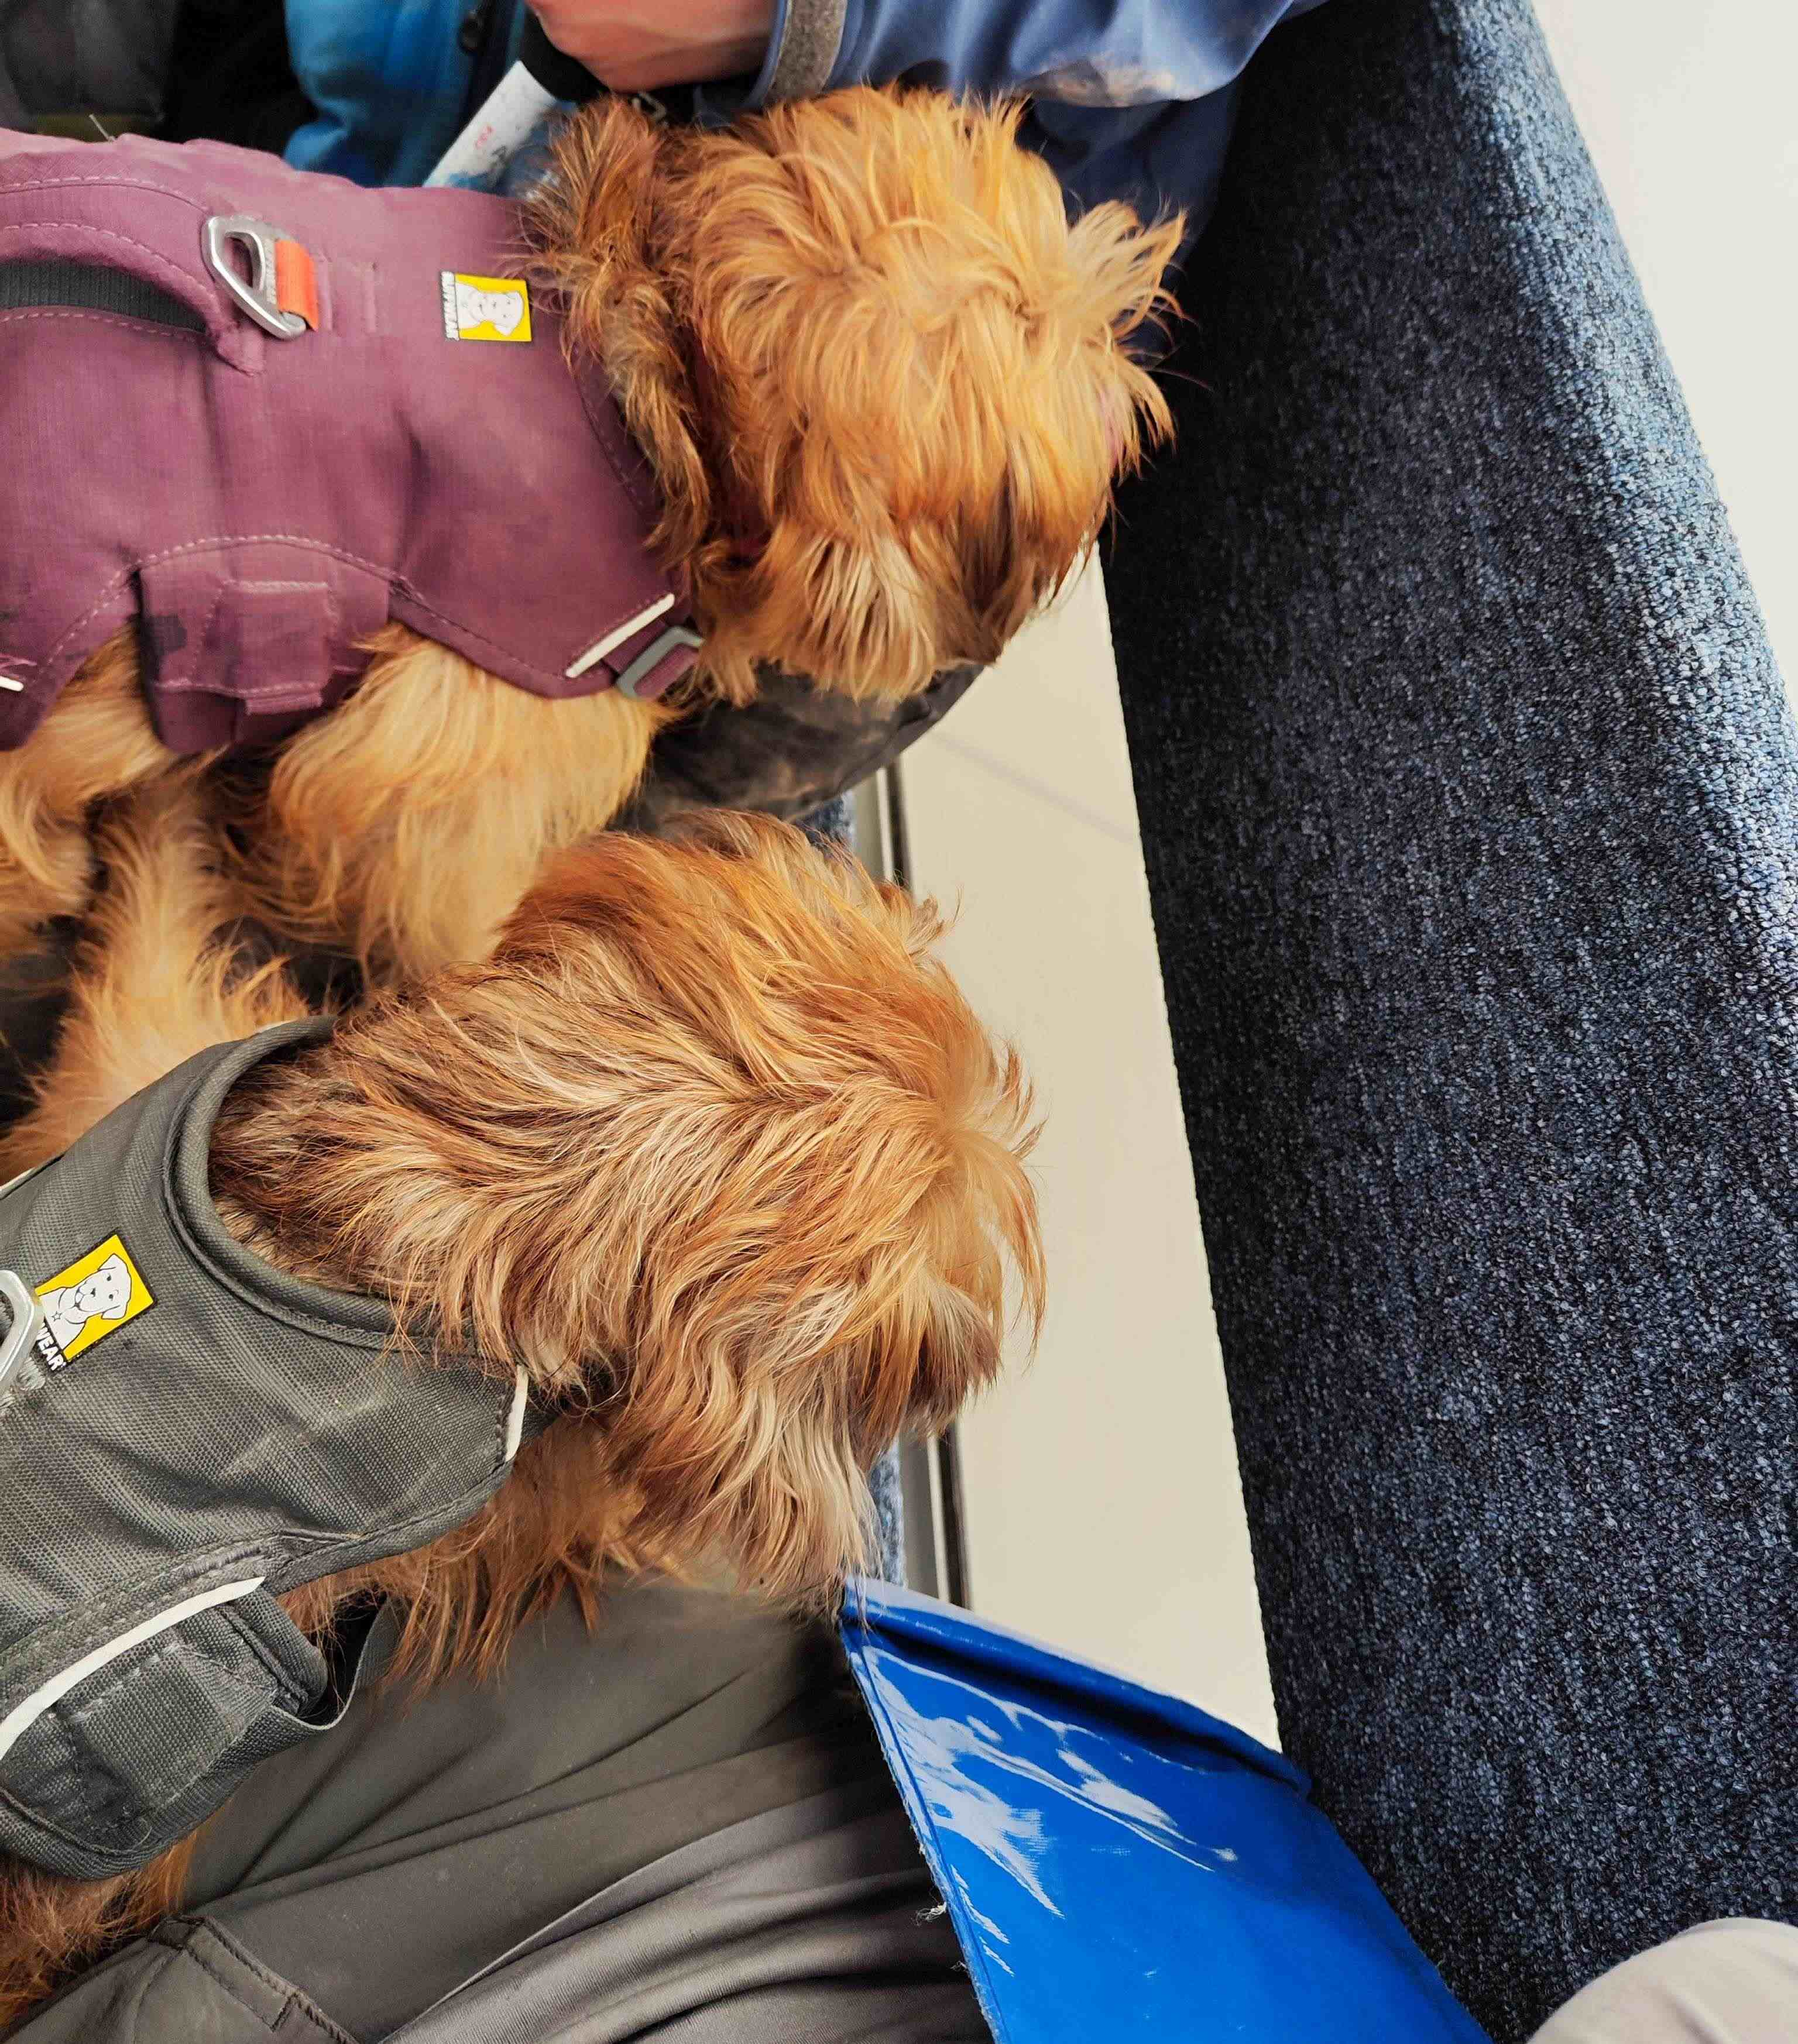
\includegraphics[width=0.4\linewidth]{../pics/IMG_20240830_170232.jpg}
	\caption{Собачки постигают новый для себя вид транспорта}
	\label{fig:IMG_20240830_170232.jpg}
\end{figure}

 Спустившись в поляну Азау, оплачиваем безбилетный проезд в закрытой , но приоткрывшейся специально для нас кассе. С нас взяли стоимость спуска с самой верхней станции канатки~--- 1200~\faRub~с человека. Сообщаем в МКК, МЧС и координатору о завершении машрута. На этом горная часть нашего путешествия завершается.

\begin{figure}[h!]
	\centering
	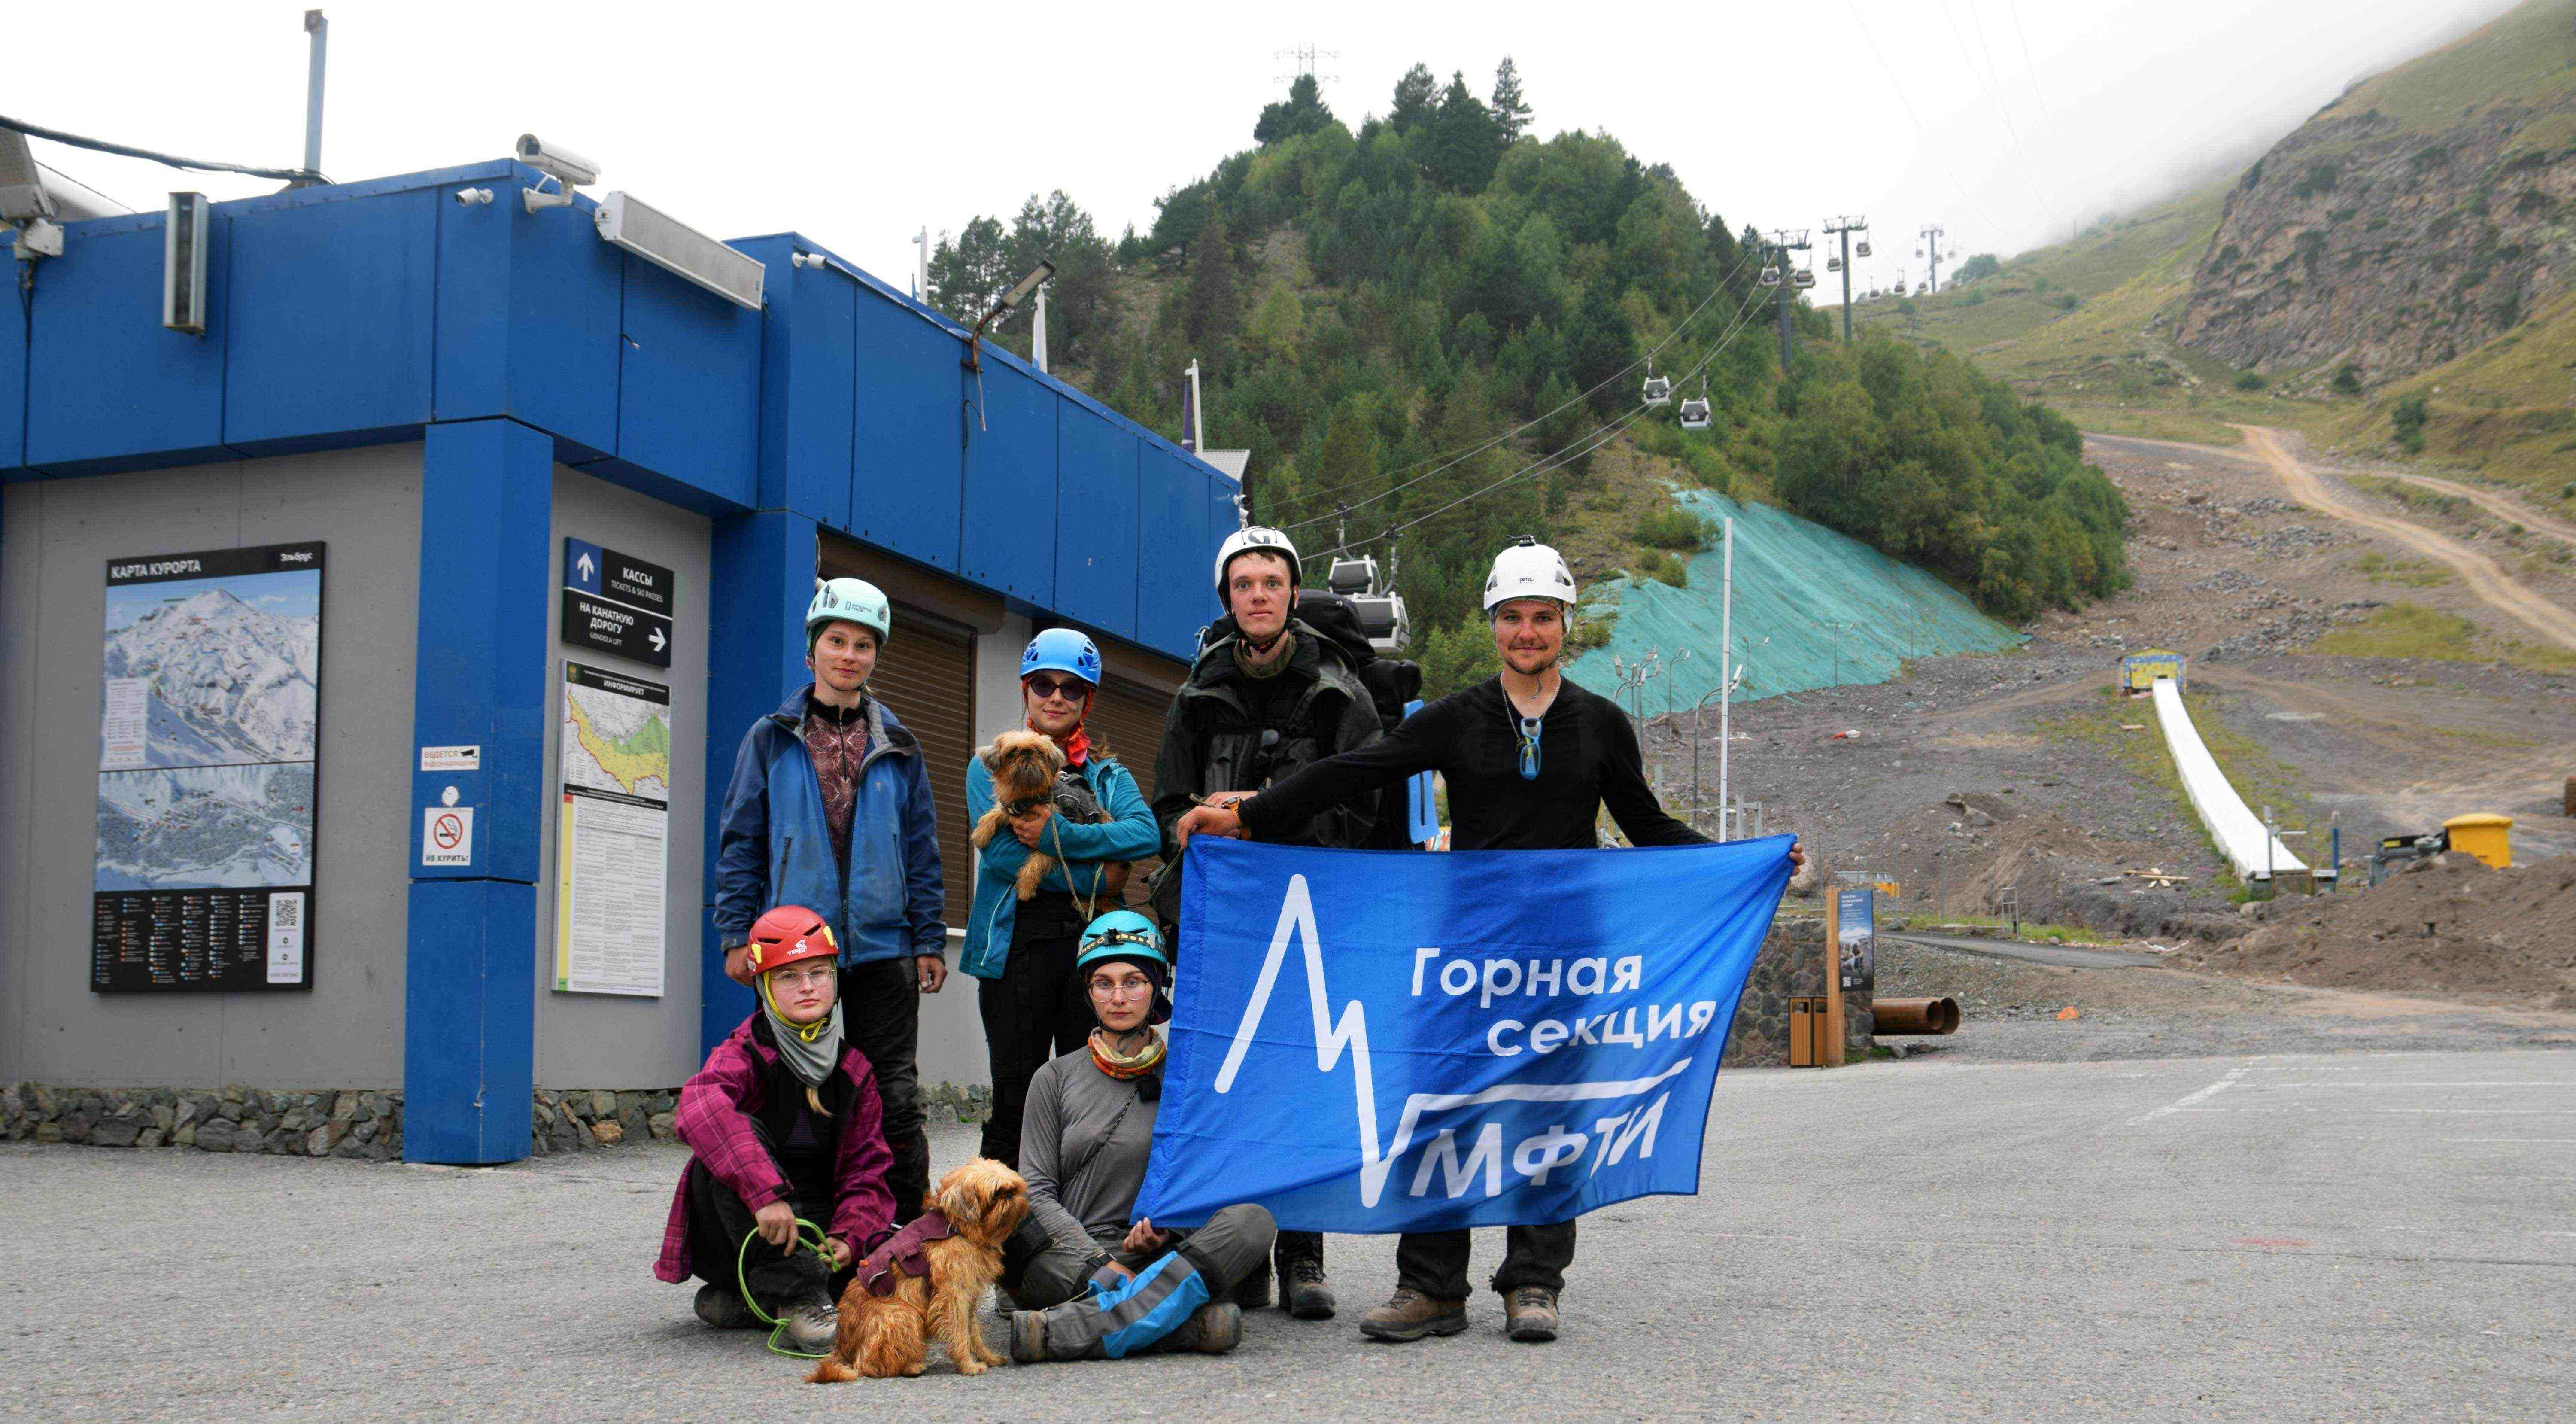
\includegraphics[width=0.7\linewidth]{../pics/group_finish.jpg}
	\caption{Конец путешествия, поляна Азау}
	\label{fig:group_finish}
\end{figure}

Остаток времени до прибытия трансфера проводим в одной из кафешек поляны Азау.
В 20:00 нас встречает микроавтобус и везёт нас до железнодородного вокзала Минеральных Вод, где мы встречаемся с участниками, покинувшими нас в Хурзуке. Как только садимся в автобус, начинаются дождь с грозой и градом, которыми пугал наш координатор, сообщая прогноз погоды. После полуночи загружаемся в поезд и катим домой!


\begin{table}[h!]
	\centering
	\begin{tabular}{|c|c|c|c|c|c|} 
		\hline 
		Этап & ЧХВ \\ 	
		\hline 
		Подход от слияния рек к каньону реки Уллукам		& 03:02\\
		Подъём по крутому травянистому склону до& 01:06 \\ выполаживания 
		Подход к месту ночёвки & 00:40 \\
		Подъём на седловину перевала Хотютау & 02:38\\
		Спуск с седловины до ледовых полей& 00:25\\
		Спуск по леднику до срединной морены & 01:50\\
		Обход зоны трещин, подход к озеру Эльбрусское& 01:00\\
		Спуск до ст. Кругозор & 00:40 \\
			
		\hline
		\textsc{Полное время подъёма на перевал  }& 07:26\\
		\textsc{Полное время спуска с перевала }& 03:55 \\
		\textsc{Полное время прохождения перевала }& 11:21 \\
		\hline
	\end{tabular}
	\caption{Расклад времени, пер. Хотютау}
\end{table}

\paragraph{Выводы и рекомендации:} ок


\clearpage